% ==============================================================
%  MEMORIA TFG — Tipo II
%  Diseño y Desarrollo de una Plataforma Software para la
%  Optimización de Comunidades Energéticas
%
%  Alumno : Roberto Rodríguez Núñez
%  Titora : Eva Mª Lorenzo Iglesias
%  Cotitor: Pedro Celard Pérez
%  Centro : ESEI — Universidade de Vigo  |  Curso 2024/2025
%
%  ESTRUCTURA: Tipo II, mapeo 1:1 con los apartados 5.7–5.17 de la
%  guía ESEI. El núcleo técnico (punto 5.11 "Marco teórico/práctico.
%  Ferramentas") es el Capítulo 5 único, con tres secciones-pilar
%  (5.1 Fundamentos+Herramientas, 5.2 Ingeniería de Datos, 5.3 Motor).
%  Numeración limitada a 3 niveles (secnumdepth=2): los hitos
%  experimentales (DQN-A…, SAC-A…) van como encabezados sin numerar.
% ==============================================================

\documentclass[12pt, a4paper, twoside]{report}

\usepackage[utf8]{inputenc}
\usepackage[T1]{fontenc}
\usepackage{lmodern}        % glifo de € y mejor cobertura T1
\usepackage{textcomp}
\usepackage[spanish]{babel}
% babel-spanish redefine \% con un pegamento que rompe el modo matemático
% (\,\% dentro de $...$). Restauramos un \% neutro en ambos modos.
\AtBeginDocument{\def\%{\char37\relax}}
\usepackage{amsmath, amssymb}
\usepackage{siunitx}
\sisetup{output-decimal-marker={,}, group-separator={.}}
\usepackage{microtype}
\usepackage[top=2.5cm, bottom=2.5cm, inner=3cm, outer=2.5cm]{geometry}
\usepackage{setspace}
\onehalfspacing
\usepackage{parskip}
\setlength{\parindent}{0pt}
\setlength{\parskip}{6pt plus 2pt minus 1pt}

% ── Profundidad de numeración y de índice ─────────────────────
% secnumdepth=2 -> se numera hasta subsection (X.Y.Z, tres números).
% subsubsection y paragraph quedan como encabezados en negrita SIN
% numerar. Esto elimina los 5.3.2.2.1 manteniendo la estructura.
\setcounter{secnumdepth}{2}
\setcounter{tocdepth}{2}

\usepackage{fancyhdr}
\pagestyle{fancy}
\fancyhf{}
\fancyhead[LE,RO]{\small\thepage}
\fancyhead[RE]{\small\nouppercase{\leftmark}}
\fancyhead[LO]{\small\nouppercase{\rightmark}}
\renewcommand{\headrulewidth}{0.4pt}
\fancypagestyle{plain}{
  \fancyhf{}
  \fancyfoot[C]{\small\thepage}
  \renewcommand{\headrulewidth}{0pt}
}

\usepackage{titlesec}
\titleformat{\chapter}[display]
  {\normalfont\Large\bfseries}
  {\chaptertitlename\ \thechapter}{16pt}{\Huge}
\titlespacing*{\chapter}{0pt}{-10pt}{30pt}

\usepackage{booktabs, array, longtable, tabularx}
\newcolumntype{L}[1]{>{\raggedright\arraybackslash}p{#1}}
\newcolumntype{C}[1]{>{\centering\arraybackslash}p{#1}}
\usepackage{graphicx, caption, subcaption, float}
\usepackage{enumitem}
\usepackage{tocloft}
\renewcommand{\cftchapfont}{\bfseries}
\renewcommand{\cftchappagefont}{\bfseries}
\setlength{\cftbeforechapskip}{6pt}

\usepackage{xcolor}
\definecolor{codebg}{RGB}{248,248,248}
\definecolor{codeframe}{RGB}{210,210,210}
\definecolor{kw}{RGB}{0,0,180}
\definecolor{cmt}{RGB}{100,100,100}
\definecolor{str}{RGB}{163,21,21}
\usepackage{listings}
\lstset{
  backgroundcolor=\color{codebg}, frame=single,
  rulecolor=\color{codeframe},
  basicstyle=\small\ttfamily,
  keywordstyle=\color{kw}\bfseries,
  commentstyle=\color{cmt}\itshape,
  stringstyle=\color{str},
  breaklines=true, captionpos=b,
  numbers=left, numberstyle=\tiny\color{gray},
  numbersep=8pt, showstringspaces=false,
  xleftmargin=15pt, language=Python
}

% Caja reutilizable para huecos de figura/diagrama pendientes
\newcommand{\figpend}[2][0.92\textwidth]{%
  \fbox{\parbox{#1}{\centering\vspace{2.6cm}\textit{#2}\vspace{2.6cm}}}}

\usepackage[hidelinks, breaklinks=true]{hyperref}
\usepackage{pdfpages}
\usepackage{cleveref}
\usepackage{natbib}
\bibliographystyle{plainnat}

\usepackage[acronym, toc, nonumberlist]{glossaries}
\makeglossaries
\newacronym{rl}{RL}{Aprendizaje por Refuerzo (\textit{Reinforcement Learning})}
\newacronym{sac}{SAC}{Actor-Crítico Suave (\textit{Soft Actor-Critic})}
\newacronym{dqn}{DQN}{Red Q Profunda (\textit{Deep Q-Network})}
\newacronym{ppo}{PPO}{Optimización de Política Proximal (\textit{Proximal Policy Optimization})}
\newacronym{td3}{TD3}{Gradiente de Política Determinista Profundo con Doble Retardo (\textit{Twin Delayed Deep Deterministic Policy Gradient})}
\newacronym{ddpg}{DDPG}{Gradiente de Política Determinista Profundo (\textit{Deep Deterministic Policy Gradient})}
\newacronym{mpc}{MPC}{Control Predictivo Basado en Modelos (\textit{Model Predictive Control})}
\newacronym{lp}{LP}{Programación Lineal (\textit{Linear Programming})}
\newacronym{ems}{EMS}{Sistema de Gestión Energética (\textit{Energy Management System})}
\newacronym{bess}{BESS}{Sistema de Almacenamiento de Energía en Baterías (\textit{Battery Energy Storage System})}
\newacronym{lfp}{LFP}{Litio Hierro Fosfato (\textit{Lithium Iron Phosphate})}
\newacronym{pvpc}{PVPC}{Precio Voluntario para el Pequeño Consumidor}
\newacronym{soc}{SoC}{Estado de Carga (\textit{State of Charge})}
\newacronym{etl}{ETL}{Extracción, Transformación y Carga (\textit{Extract, Transform, Load})}
\newacronym{api}{API}{Interfaz de Programación de Aplicaciones (\textit{Application Programming Interface})}
\newacronym{ccee}{CCEE}{Comunidad Energética de Autoconsumo}
\newacronym{fv}{FV}{Fotovoltaico}
\newacronym{mdp}{MDP}{Proceso de Decisión de Markov (\textit{Markov Decision Process})}
\newacronym{sb3}{SB3}{Stable-Baselines3}
\newacronym{saas}{SaaS}{Software como Servicio (\textit{Software as a Service})}
\newacronym{mer}{MER}{Modelo Entidad-Relación}
\newacronym{onnx}{ONNX}{Open Neural Network Exchange}

\hypersetup{
  pdftitle={Diseño y Desarrollo de una Plataforma Software para la Optimización de Comunidades Energéticas},
  pdfauthor={Roberto Rodríguez Núñez},
  pdfsubject={TFG Tipo II — ESEI, Universidade de Vigo, 2025}
}

% ==============================================================
\begin{document}
% ==============================================================

% ── PORTADA OFICIAL ───────────────────────────────────────────
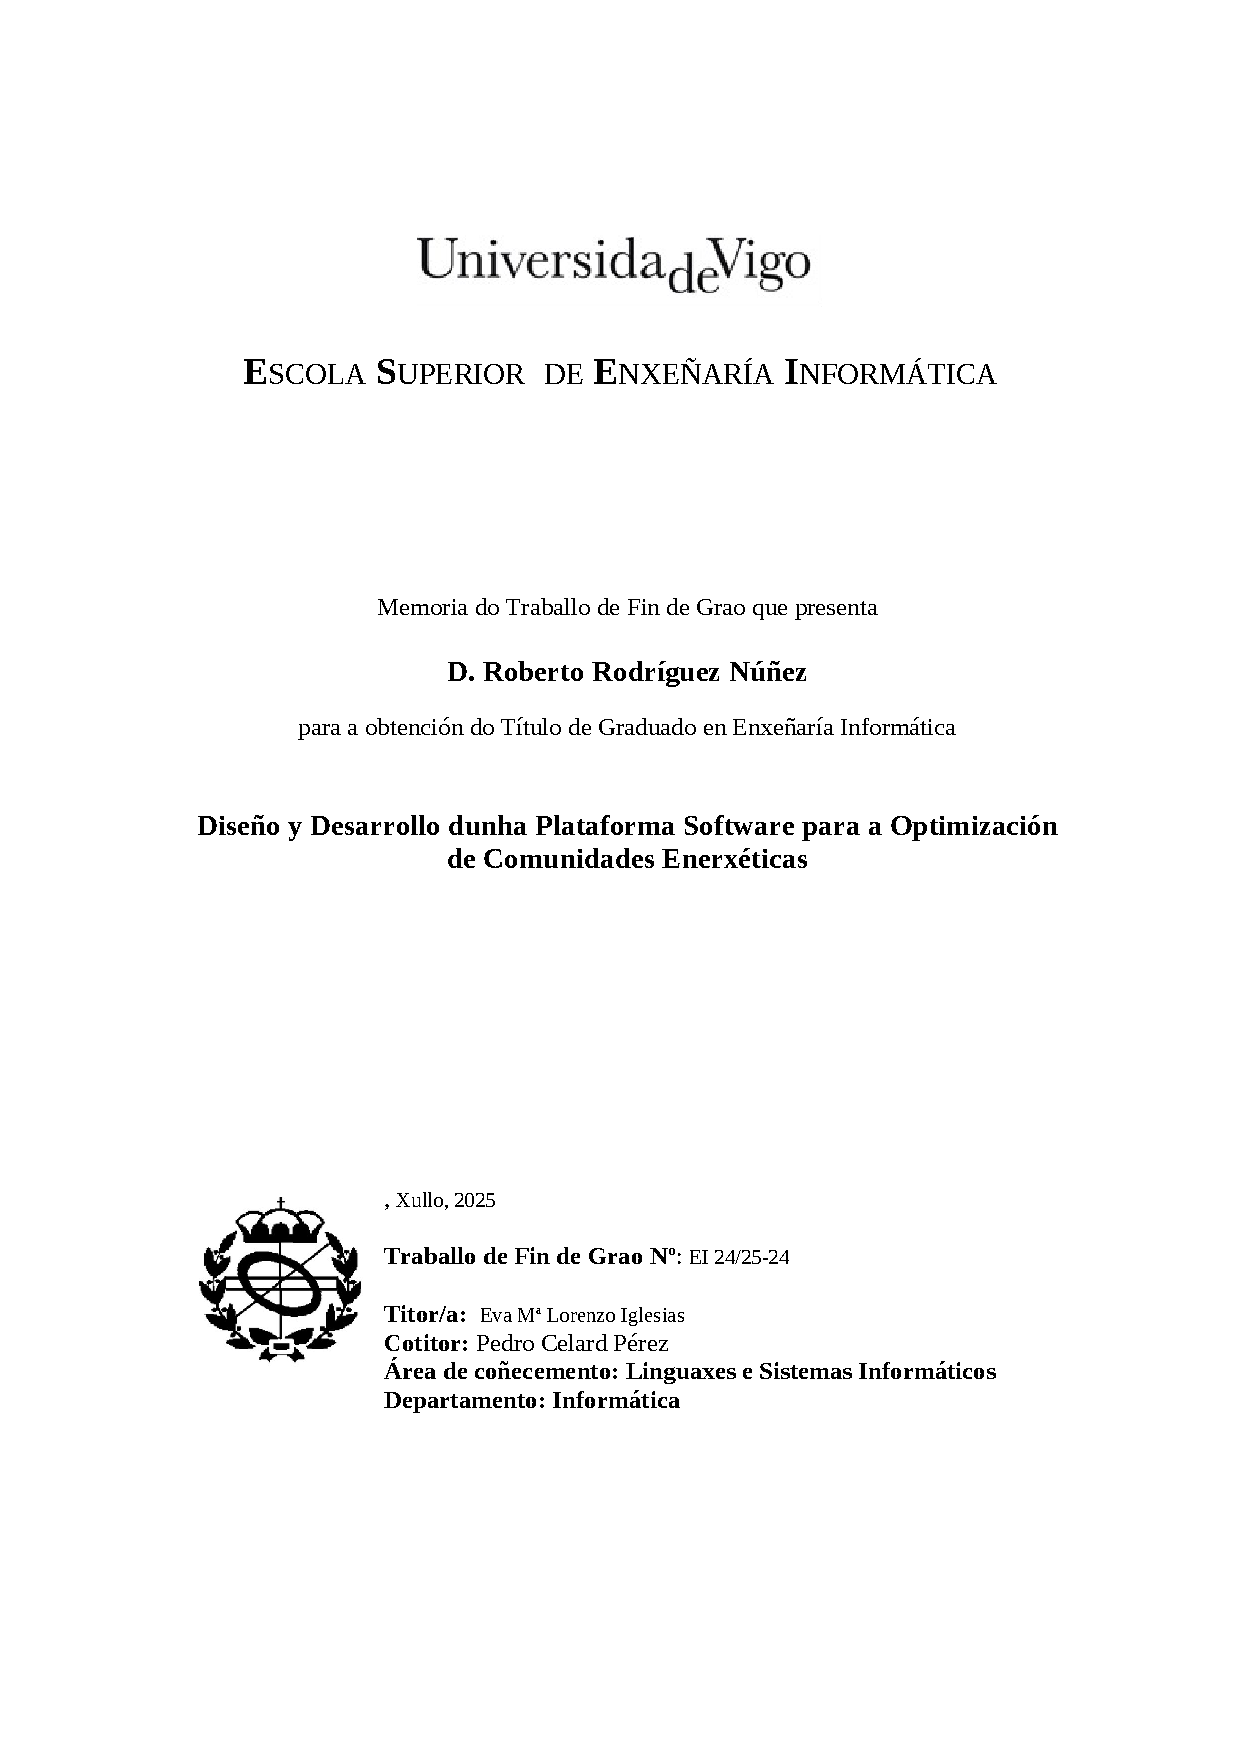
\includepdf[pages=1, fitpaper=true]{portada_oficial}

% ── PRELIMINARES ──────────────────────────────────────────────
\pagenumbering{roman}
\setcounter{page}{1}

\chapter*{Dedicatoria}
\addcontentsline{toc}{chapter}{Dedicatoria}
\thispagestyle{plain}
\vspace*{4cm}
\begin{flushright}\textit{[Espacio reservado]}\end{flushright}

\chapter*{Agradecimientos}
\addcontentsline{toc}{chapter}{Agradecimientos}
\thispagestyle{plain}
[Espacio reservado para agradecimientos]

% ── Resumen ───────────────────────────────────────────────────
\chapter*{Resumen}
\addcontentsline{toc}{chapter}{Resumen}
\thispagestyle{plain}

El actual marco regulatorio del autoconsumo colectivo en España, consolidado
mediante el Real Decreto 244/2019, ha abierto una oportunidad para que las
comunidades de pequeña escala gestionen de forma autónoma su energía
fotovoltaica. Sin embargo, las soluciones de gestión inteligente disponibles
suelen ser cerradas y propietarias y están concebidas mayoritariamente para el
almacenamiento individual o industrial; las pocas orientadas al caso comunitario
rara vez resultan accesibles o adaptables a una comunidad rural de pequeña
escala bajo el RD 244/2019, ni validan de forma transparente el beneficio que
aporta su controlador frente a una referencia bien calibrada.

Este trabajo investiga, diseña e implementa un motor de decisión inteligente
basado en aprendizaje por refuerzo para la optimización económica de la batería
comunitaria en una comunidad energética de autoconsumo fotovoltaico colectivo.
Tras un proceso documentado de experimentación con los algoritmos \acrshort{dqn}
y \acrshort{ppo}, se diseña e implementa el controlador Residual \acrshort{sac}
sobre un \acrshort{mpc} base, arquitectura híbrida que resuelve los problemas de
arranque en frío y cuantización que impidieron a los candidatos anteriores
superar el \textit{baseline} competitivo, que en la configuración final se
sitúa en $+47{,}64$\,€/semana.

El motor se integra en una plataforma software de tipo \acrshort{saas} con
gemelo digital de la instalación, módulo de ingeniería de datos con fuentes
oficiales (ESIOS, PVGIS) y capa de visualización diferenciada por rol
(Superadmin y Usuario de la comunidad). El sistema implementa la capa de
planificación horaria (Nivel~3) del control jerárquico estándar para sistemas
de almacenamiento, replicando la lógica de despacho horario utilizada por
los agregadores energéticos en el mercado diario de OMIE.

\textbf{Palabras clave:} comunidades energéticas, autoconsumo colectivo,
aprendizaje por refuerzo, Soft Actor-Critic, control predictivo basado en
modelos, RD 244/2019, optimización energética.

\chapter*{Abstract}
\addcontentsline{toc}{chapter}{Abstract}
\thispagestyle{plain}

Spain's regulatory framework for collective self-consumption, established by
Royal Decree 244/2019, has created an opportunity for small-scale communities
to autonomously manage their photovoltaic energy. However, the lack of
accessible tools forces reliance on static sharing models that underutilise
the installation's most valuable asset: the community battery.

This work investigates, designs and implements an intelligent decision engine
based on reinforcement learning for the economic optimisation of the community
battery in a collective photovoltaic self-consumption energy community. After
a documented experimentation process with DQN and PPO, the Residual SAC
controller over an MPC base is designed and implemented, a hybrid architecture
that resolves the cold-start and quantisation problems that prevented previous
candidates from surpassing the competitive baseline of
$+47.64$\,€/week.

\textbf{Keywords:} energy communities, collective self-consumption,
reinforcement learning, Soft Actor-Critic, model predictive control,
RD 244/2019.

\tableofcontents
\listoffigures
\addcontentsline{toc}{chapter}{Índice de figuras}
\listoftables
\addcontentsline{toc}{chapter}{Índice de tablas}
\printglossary[type=acronym, title={Glosario de Acrónimos}]

% ── CUERPO ────────────────────────────────────────────────────
\pagenumbering{arabic}
\setcounter{page}{1}

% ==============================================================
\chapter{Introducción}
\label{chap:intro}
% ==============================================================

\section{Contexto y Problemática}

La transición energética hacia un modelo descarbonizado sitúa al autoconsumo
fotovoltaico colectivo como uno de los instrumentos más prometedores para
democratizar la generación de energía renovable a nivel ciudadano. El Real
Decreto 244/2019 consolidó en España el marco regulatorio que permite a varias
unidades de consumo compartir una instalación de generación fotovoltaica y
distribuir los excedentes entre sus participantes mediante coeficientes de
reparto horarios. Este mecanismo abre la puerta a un modelo energético más
justo y autónomo, especialmente en el entorno rural.

Sin embargo, la puesta en práctica de este potencial choca con una realidad
técnica. Existen soluciones comerciales de gestión energética e incluso
productos que abordan el almacenamiento compartido, pero la mayoría son cerradas
y propietarias —difíciles de auditar y de adaptar— y están diseñadas para el
almacenamiento individual o industrial, donde la batería responde a un único
punto de consumo. Las que sí contemplan el caso comunitario rara vez se ajustan
al modelo de liquidación agregada que impone el RD 244/2019 ni resultan
asequibles para una comunidad rural de pequeña escala, y casi nunca documentan
de forma transparente cuánto beneficio económico aporta realmente su controlador
frente a una referencia bien calibrada. La batería de una comunidad de
autoconsumo colectivo plantea, por tanto, un problema distinto: un único activo
debe gestionarse de forma centralizada para el balance agregado de todos los
participantes, y queda infrautilizada sin una política de carga y descarga que
explote la variabilidad horaria del precio de la energía en el mercado español.

La variabilidad del precio PVPC, que en 2022 alcanzó \num{0,50}\,€/kWh en horas
pico y valores cercanos a cero en horas valle, ofrece un margen de arbitraje
que solo un motor de decisión con capacidad predictiva puede explotar. El
presente trabajo aborda este problema desde una perspectiva dual: investigadora,
al desarrollar y comparar algoritmos de aprendizaje por refuerzo aplicados a
este dominio; e ingenieril, al integrar el motor resultante en una plataforma
software accesible para comunidades rurales de pequeña escala.

\section{Posicionamiento en el Control Jerárquico Estándar}

El sistema implementa la \textbf{capa de planificación horaria (Nivel~3)} del
control jerárquico estándar para sistemas de almacenamiento de energía. Esta
capa opera con horizonte de 24 horas y resolución horaria, determinando la
estrategia económicamente óptima de carga y descarga en función del pronóstico
de precios, generación y consumo. La integración con la capa de control
supervisorio (Nivel~2, SCADA) y la capa de control en tiempo real (Nivel~1,
BMS) queda como trabajo futuro para el despliegue en instalaciones reales.

Desde la perspectiva del mercado eléctrico, la arquitectura replica la capa de
despacho horario utilizada por los agregadores energéticos en el mercado diario
español (OMIE). La participación en mercados intradiarios de OMIE y en servicios
de balance de REE —que operan en horizontes sub-horarios— queda como extensión
natural hacia una arquitectura de gestión energética multi-capa completa.

\section{Estructura del Documento}

El documento sigue la estructura del Tipo~II de la Guía de Elaboración del TFG
de la ESEI. El Capítulo~\ref{chap:objetivos} define los objetivos. El
Capítulo~\ref{chap:antecedentes} revisa los antecedentes y el contexto del
problema. El Capítulo~\ref{chap:solucion} resume la solución propuesta y la
metodología. El Capítulo~\ref{chap:marco}, marco práctico y herramientas
empleadas, constituye el núcleo técnico del trabajo: desarrolla los fundamentos
teóricos y el \textit{stack} tecnológico (Sección~\ref{sec:fundamentos}), la
ingeniería de datos y el gemelo digital físico-económico de la comunidad
(Sección~\ref{sec:datos}), el motor de decisión (Sección~\ref{sec:motor}), su
exportación a producción (Sección~\ref{sec:onnx}) y la plataforma SaaS
(Sección~\ref{sec:saas}). Los Capítulos~\ref{chap:planificacion}
a~\ref{chap:futuro} completan la documentación con planificación, aportaciones,
conclusiones y trabajo futuro.

% ==============================================================
\chapter{Objetivos}
\label{chap:objetivos}
% ==============================================================

Este trabajo se articula en torno a una \textbf{pregunta de investigación}:

\begin{quote}
\itshape ¿Puede un controlador basado en aprendizaje por refuerzo superar a los
controladores convencionales —desde las reglas heurísticas hasta el control
predictivo basado en modelos— en la optimización económica de la batería de una
comunidad energética de autoconsumo fotovoltaico colectivo bajo el RD 244/2019?
\end{quote}

De ella se deriva la \textbf{hipótesis de trabajo} que la experimentación
buscará contrastar: un agente de \acrshort{rl} que opera de forma autónoma
iguala, pero no supera de forma consistente, a un \acrshort{mpc} bien calibrado;
en cambio, una arquitectura híbrida que aprende correcciones residuales sobre
ese MPC sí logra superarlo, conservando como garantía de suelo el rendimiento
del propio MPC. Aceptar o rechazar esta hipótesis —y cuantificar el margen de
mejora— es el hilo conductor de la fase experimental (Sección~\ref{sec:motor}).

El objetivo central del presente trabajo es el diseño, implementación y
validación experimental de un motor de decisión basado en aprendizaje por
refuerzo para la optimización económica de la batería comunitaria en una
comunidad energética de autoconsumo fotovoltaico colectivo, operando bajo el
marco regulatorio del RD 244/2019, e integrado en una plataforma software
accesible orientada a comunidades rurales de pequeña escala.

\section{Objetivos Generales}

\begin{enumerate}[label=\textbf{OG\arabic*.}]
  \item Investigar y comparar algoritmos de aprendizaje por refuerzo aplicados
    a la gestión de sistemas de almacenamiento de energía, con especial atención
    a su capacidad para superar un \textit{baseline} de control predictivo bien
    calibrado.
  \item Diseñar e implementar un gemelo digital físico-económico de una comunidad
    energética, calibrado con datos reales de fuentes oficiales (ESIOS, PVGIS),
    que sirva como entorno de entrenamiento y evaluación reproducible.
  \item Seleccionar, justificar e implementar el algoritmo de control más adecuado
    tras experimentación documentada con candidatos alternativos.
  \item Integrar el motor de decisión en una plataforma software accesible que
    democratice la gestión energética inteligente para comunidades rurales.
\end{enumerate}

\section{Objetivos Específicos}

\begin{enumerate}[label=\textbf{OE\arabic*.}]
  \item Construir el pipeline \acrshort{etl} reproducible que integre datos de
    consumo normativo (ESIOS 2.0TD), generación \acrshort{fv} (PVGIS) y precios
    de mercado (PVPC e indicador de compensación simplificada) en un dataset
    unificado de 22.646 horas.
  \item Implementar el simulador físico-económico con modelo de degradación no
    lineal de batería LFP y modelo económico asimétrico coherente con el
    RD 244/2019.
  \item Implementar el controlador \acrshort{mpc} con horizonte deslizante de
    24 horas como cota teórica (pronóstico oráculo) y como \textit{baseline}
    competitivo (pronóstico realista con ruido AR(1)).
  \item Experimentar con \acrshort{dqn} y \acrshort{ppo} como algoritmos
    candidatos, documentando su rendimiento y sus limitaciones estructurales.
  \item Diseñar e implementar el controlador Residual \acrshort{sac} con
    protocolo de inicialización con demostraciones del MPC, y validar
    experimentalmente que supera al \textit{baseline} competitivo.
  \item Desarrollar una suite de tests automatizados que garantice los
    invariantes físicos y económicos del simulador y la reproducibilidad
    de los experimentos.
\end{enumerate}

\section{Alcance}

El trabajo cubre el diseño, implementación y validación experimental del motor
de decisión sobre datos históricos simulados. La integración con APIs de datos
en tiempo real está diseñada pero no activada en el prototipo actual. El
despliegue en hardware físico y la integración con datos de viviendas reales
constituyen extensiones naturales en el trabajo futuro.

% ==============================================================
\chapter{Antecedentes y Contexto}
\label{chap:antecedentes}
% ==============================================================

\section{Marco Regulatorio del Autoconsumo Colectivo en España}
\label{sec:marco_regulatorio}

El autoconsumo colectivo en España, en transposición de la normativa europea
sobre energías renovables y mercado interior de la electricidad, se regula
mediante el \textbf{Real Decreto 244/2019}~\citep{RD244_2019}, que establece las condiciones
administrativas, técnicas y económicas del autoconsumo e introduce el mecanismo
de \textbf{compensación simplificada de excedentes}, posteriormente reforzado
por el Real Decreto-ley 7/2025~\citep{RDL7_2025}.

El mecanismo realiza una liquidación económica hora a hora del intercambio de
energía entre la comunidad y la red. En cada hora se compara la generación
fotovoltaica total con el consumo total de la comunidad, y pueden darse dos
situaciones. Si la generación es \textbf{menor} que el consumo, la comunidad
autoconsume toda la energía solar producida (que no se factura, pues sustituye
energía que habría que comprar) y adquiere de la red el déficit restante al
precio de compra PVPC. Si la generación es \textbf{mayor} que el consumo, la
comunidad autoconsume la parte que cubre su demanda y vierte el excedente
sobrante a la red, recibiendo por él una compensación al precio mayorista.

Al final del periodo de facturación, la compensación acumulada por los
excedentes vertidos se descuenta del importe de la energía comprada. Esta
compensación está limitada: puede reducir la factura hasta cero, pero nunca
generar un saldo a favor del consumidor. La energía entra y sale físicamente de
la red con normalidad en ambas direcciones; el mecanismo de compensación es
únicamente la liquidación económica de ese intercambio.

\textbf{Modelo de comunidad adoptado.} El caso de estudio es una
\textbf{ecocomunidad rural} de quince viviendas en \textbf{parcelas colindantes
de titularidad privada}, organizada como \textbf{cooperativa} que actúa como
titular único del suministro eléctrico. La interconexión entre la generación
distribuida de cada parcela y la batería comunitaria se realiza mediante una
\textbf{red interior privada} —cableado propio bajo servidumbre de paso entre
fincas colindantes—, de modo que la energía fluye internamente \emph{sin
atravesar la red de distribución pública}, y la comunidad se presenta ante el
sistema eléctrico a través de un \textbf{único contador frontera}.

Bajo esta topología, el \textbf{balance horario agregado} entre el consumo y la
generación totales de la comunidad es \emph{exactamente} lo que registra el
contador frontera y constituye la única factura eléctrica oficial. Esto justifica
que el simulador modele la comunidad como \textbf{nodo agregado} no como una
simplificación, sino como una \textbf{correspondencia físicamente exacta}: el
balance agregado sobre el que decide el controlador \emph{es} la factura que se
optimiza. El reparto de ese coste único entre las viviendas es una operación
\textbf{interna} de la cooperativa —repercusión de gasto común medido por
subcontadores privados, sin reventa de energía conforme a la Ley 24/2013—, no una
facturación regulada vivienda a vivienda; el coeficiente de reparto es, por tanto,
una \textbf{clave interna} que distribuye coste y ahorro entre los socios, no el
coeficiente reglamentario del autoconsumo colectivo.

\textbf{Por qué no el autoconsumo colectivo estándar.} La alternativa
reglamentaria directa, el \textbf{autoconsumo colectivo a través de red} del
RD 244/2019, \emph{no} produce un nodo agregado real: no existe conexión física
entre viviendas, sino que la distribuidora reparte la generación —y la descarga
de la batería— entre los distintos CUPS mediante \textbf{coeficientes fijos}
($\text{ENG}_{h,i}=\beta_{h,i}\cdot\text{ENG}_h$) y netea \emph{cada vivienda por
separado}. Esto introduce dos ineficiencias que el modelo agregado evita:
(i) el excedente de un vecino se vierte a la red a precio mayorista mientras otro
compra su déficit a PVPC en la misma hora, sin compensación cruzada; y (ii) la
batería compartida se descargaría repartida por coeficientes \emph{ciegos},
ajenos a quién demanda realmente la energía, desperdiciando su valor. La red
interior privada de la cooperativa elimina ambas, permitiendo que el controlador
asigne cada flujo a quien lo necesita.

\textbf{Condiciones de aplicabilidad y encuadre regulatorio.} Esta
correspondencia exacta exige condiciones concretas, que se asumen explícitamente
y se discuten como limitación (Sección~\ref{sec:limitaciones}): parcelas
colindantes sin vía de dominio público interpuesta —por la que no es legal tender
cableado privado—, titularidad única del suministro por la cooperativa y renuncia
de los vecinos al contrato individual con comercializadora. Conviene precisar que
este modelo \emph{no} es una figura regulada llave en mano: las Redes de
Distribución Cerradas (Real Decreto 1183/2020 y Real Decreto 314/2023) están
reservadas a entornos industriales —solo admiten consumo residencial como
excepción marginal y ligada a la industria, manteniendo además cada consumidor su
comercializadora—, por lo que el escenario aquí adoptado se sostiene jurídicamente
como \emph{red interior de un único consumidor} (la cooperativa), no como red de
distribución cerrada. Su viabilidad económica se apoya en los programas de
incentivos a comunidades energéticas con almacenamiento (Programa CE~IMPLEMENTA,
Orden TED/764/2024, IDAE), que exigen sistema de almacenamiento de forma
obligatoria.

La característica que condiciona el diseño del motor de decisión es la asimetría
de precios: el precio de venta de excedentes (mayorista, indicador 1739 de
ESIOS) es sistemáticamente inferior al de compra (PVPC, indicador 1001), que
incluye peajes y cargos del sistema. Por ello, maximizar el autoconsumo interno
es siempre más rentable que maximizar la venta de excedentes.

\section{El Problema de la Gestión de Baterías en Comunidades Energéticas}

La inclusión de un sistema de almacenamiento de energía en baterías
(\acrshort{bess}) en una comunidad de autoconsumo introduce un problema de
decisión secuencial bajo incertidumbre: en cada hora del día, el gestor debe
decidir cuánta energía cargar o descargar de la batería considerando el precio
actual de la energía, la generación solar disponible, el consumo esperado de
las viviendas y el estado de carga actual de la batería.

Este problema tiene tres características que lo hacen especialmente adecuado
para técnicas de optimización avanzada. En primer lugar, las decisiones son
secuencialmente dependientes: cargar la batería ahora reduce el margen de carga
disponible en las próximas horas. En segundo lugar, existe incertidumbre sobre
el futuro: ni el consumo, ni la generación solar, ni siquiera el precio de la
energía son perfectamente predecibles con horas de antelación. En tercer lugar,
el horizonte de decisión relevante es de 24 horas, suficiente para que el precio
varíe entre máximos y mínimos que crean oportunidades de arbitraje temporal. El
precio, además, solo se conoce con exactitud de forma parcial: REE publica el
\acrshort{pvpc} del día siguiente a partir de las 20:30\,h, de modo que dentro
del horizonte de 24 horas las primeras horas son ciertas y las posteriores deben
estimarse, diferencia que motiva el modelo de pronóstico en tres capas empleado
en este trabajo (Sección~\ref{sec:motor}).

La estrategia realmente óptima no es evidente a priori: depende de la
interacción entre generación, consumo, precio y degradación, todos ellos
sujetos a incertidumbre dentro del horizonte de 24 horas, y es precisamente lo
que el motor de decisión debe aprender o calcular.

\section{El Espacio de Acciones: Discreto frente a Continuo}

La aplicación de aprendizaje por refuerzo a la gestión de sistemas de
almacenamiento de energía ha experimentado un crecimiento notable en la última
década, desde los trabajos fundacionales de \citet{Mnih2015} sobre
\acrshort{dqn}. Su aplicación a los sistemas energéticos y a la respuesta de
la demanda está ampliamente documentada en revisiones recientes
\citep{Perera2021, Vazquez2019}. La decisión de diseño más determinante en este dominio es la
topología del espacio de acciones, que condiciona estructuralmente tanto el
algoritmo aplicable como la calidad de la política aprendida.

Un \textbf{espacio discreto} representa las decisiones de la batería como un
conjunto finito de acciones que combinan estrategia (cargar, descargar, no
actuar) con nivel de potencia. Es la representación que emplean algoritmos
basados en valor como \acrshort{dqn}, y encaja bien con la gestión eléctrica
porque la estrategia rentable suele consistir en concentrar la carga y la
descarga en los picos y valles de precio, que son decisiones de naturaleza
discreta. Su ventaja es la simplicidad y la estabilidad de entrenamiento. Su
limitación es el error de cuantización: el conjunto finito de niveles no puede
representar los ajustes de potencia intermedios que la política óptima requiere
en algunas horas. En este trabajo se experimentó con \acrshort{dqn} y también
con \acrshort{ppo} sobre el mismo espacio discreto.

Un \textbf{espacio continuo} asigna directamente la potencia neta dentro del
rango físico del inversor. Elimina por construcción el error de cuantización a
costa de requerir algoritmos de control continuo más sofisticados como
\acrshort{sac}.

\section{Estado del Arte: RL puro frente a MPC y la Arquitectura Híbrida}

El aprendizaje por refuerzo aplicado a la gestión de sistemas energéticos ha
pasado en la última década de propuestas aisladas a un cuerpo de literatura
consolidado. Revisiones sistemáticas del área \citep{Perera2021, Vazquez2019}
recogen su aplicación a la respuesta de la demanda, la climatización de
edificios, la carga de vehículos eléctricos y el arbitraje de almacenamiento, e
identifican como factores determinantes del éxito la formulación de la función
de recompensa, la eficiencia de muestreo y la capacidad de generalización entre
instalaciones. La gestión de baterías es uno de los casos más estudiados, por su
naturaleza de decisión secuencial bajo incertidumbre y por el atractivo de
aprender políticas adaptadas a patrones de precio y consumo no estacionarios sin
necesidad de un modelo explícito del sistema.

Ahora bien, el aprendizaje por refuerzo no compite en el vacío. El control
predictivo basado en modelos \citep{Rawlings2017} constituye el estado de la
práctica en el despacho económico de almacenamiento: incorpora de forma
explícita las restricciones físicas del sistema y, con un pronóstico razonable,
alcanza soluciones próximas al óptimo. Por ello, la comparación
metodológicamente exigente no enfrenta al RL contra una heurística simple, sino
contra un MPC bien calibrado. La literatura sobre esta comparación no es
concluyente: en dominios de gestión energética el RL puro tiende a igualar el
rendimiento de un MPC bien sintonizado, pero superarlo de forma consistente
resulta difícil, precisamente porque el MPC ya explota la estructura del
problema que el agente debería aprender desde cero. Es esta tensión la que
motiva el interés por las arquitecturas híbridas, que es el enfoque adoptado en
este trabajo.

La comparativa honesta del RL con controladores \acrshort{mpc} bien calibrados
muestra un panorama matizado. En el contexto regulatorio español del PVPC, un
MPC determinista correctamente sintonizado captura ya en torno al 90\,\% del
valor económico disponible mediante arbitraje diario y emparejamiento de picos
de precio. La literatura sobre arquitecturas residuales en dominios afines
(microrredes, sistemas HVAC) documenta que el margen de mejora realista que un
esquema híbrido puede aportar sobre ese MPC se sitúa típicamente entre el 4\,\%
y el 12\,\%, reduciéndose a valores más modestos cuando el MPC ya está bien
calibrado. Este margen acotado, lejos de invalidar el enfoque, define con
precisión el espacio en el que el motor de IA debe demostrar su valor.

La arquitectura híbrida MPC+RL responde a esta realidad combinando la
estabilidad y las garantías del MPC con la capacidad adaptativa del RL.
\citet{Johannink2019} propusieron el \textit{Residual Reinforcement Learning}
en el contexto del control robótico: el agente aprende únicamente las
correcciones residuales sobre un controlador base competente, aprovechando el
conocimiento encapsulado en ese controlador como punto de partida. Aplicada al
presente trabajo, esta arquitectura aporta una propiedad de \textbf{seguridad
por construcción}: como la corrección del agente está acotada, si el agente
propone una corrección nula el sistema replica exactamente el comportamiento
del MPC subyacente, eliminando el riesgo de exploración destructiva que
desaconseja el uso de RL puro en infraestructuras críticas.

La selección del algoritmo de RL continuo para calcular la corrección residual
se desarrolla en detalle en la Sección~\ref{sec:motor}, donde se justifica la
elección de \acrshort{sac} frente a las alternativas continuas (PPO, TD3, DDPG)
sobre la base de su eficiencia de muestreo y su robustez ante la alta varianza
de la recompensa económica.

\section{Soluciones Actuales para la Gestión del Almacenamiento}

La gestión de baterías con inteligencia artificial es ya una realidad, tanto en
el ámbito comercial como en proyectos de investigación: existen sistemas EMS
propietarios e incluso plataformas que abordan el almacenamiento compartido.
Ahora bien, la mayoría de estas soluciones presentan tres limitaciones para el
escenario de este trabajo. En primer lugar, son de carácter cerrado y
propietario, lo que dificulta auditarlas y adaptarlas a contextos para los que
no fueron diseñadas. En segundo lugar, están orientadas mayoritariamente al
almacenamiento individual o industrial —donde la batería responde a un único
punto de consumo— y no al nodo agregado que impone el RD 244/2019. En tercer
lugar, rara vez documentan de forma reproducible y transparente la mejora
económica que su controlador aporta frente a una referencia bien calibrada, de
modo que resulta difícil saber cuánto valor añade realmente la inteligencia
frente a un control clásico. En comunidades de pequeña escala con recursos
limitados, estas tres carencias se agravan.

La batería de una comunidad de autoconsumo colectivo plantea un problema
distinto, porque un único activo debe gestionarse de forma centralizada para el
balance agregado de todos los participantes bajo el marco del RD 244/2019. La
energía generada se reparte entre las viviendas y solo el excedente conjunto se
vierte a la red, de modo que la decisión de carga y descarga afecta a toda la
comunidad y no a un consumidor aislado. El presente trabajo se centra en este
escenario, aplicando aprendizaje por refuerzo a la optimización económica del
almacenamiento comunitario y midiendo de forma transparente la mejora que aporta
frente a un control de referencia bien calibrado.

% ==============================================================
\chapter{Resumen de la Solución Propuesta y Metodología}
\label{chap:solucion}
% ==============================================================

\section{Descripción General}

La solución propuesta es la plataforma EnergyComm, organizada en cinco capas
funcionales. La comunidad modelada comprende quince viviendas con perfil de
consumo residencial 2.0TD, una instalación fotovoltaica compartida de
\SI{42}{kWp} y una batería comunitaria de tecnología \acrshort{lfp} con capacidad
de \SI{80}{kWh} e inversor bidireccional de \SI{50}{kW}.

La \textbf{capa de datos} construye y mantiene el dataset de simulación a partir
de fuentes oficiales. La \textbf{capa del simulador} implementa el gemelo digital
físico-económico. La \textbf{capa de aprendizaje por refuerzo} contiene el
entorno Gymnasium~\citep{Gymnasium2023} y el motor de decisión. La \textbf{capa de producción}
gestiona el ciclo de vida del modelo entrenado y su exportación a formato ONNX
para su despliegue en hardware de borde. La \textbf{capa SaaS} expone los
resultados a los usuarios finales mediante una interfaz web diferenciada por
rol, con persistencia de los perfiles e histórico de la comunidad.

\begin{figure}[H]
  \centering
  \figpend{[Figura: Arquitectura de 5 capas de la plataforma EnergyComm]\\
    \textit{Exportar arquitectura\_capas.drawio $\rightarrow$ img/arquitectura\_capas.png}}
  \caption{Arquitectura de la plataforma EnergyComm organizada en cinco capas.}
  \label{fig:arquitectura}
\end{figure}

\section{Metodología}

El desarrollo sigue un ciclo iterativo de tipo Scrum con sprints semanales,
adaptado a las características de un proyecto de investigación aplicada. Las
iteraciones alternan entre el desarrollo de componentes software y la
experimentación con el motor de decisión, con validación continua mediante la
suite de tests automatizados.

Se aplica la metodología MLOps al ciclo de vida del motor de decisión:
configuración externalizada en YAML (sin \textit{magic numbers} en el código,
siguiendo principios de código limpio \citep{Martin2009}),
semillas fijas para reproducibilidad total de experimentos, versionado de modelos
entrenados y de las estadísticas de normalización (\texttt{vec\_normalize.pkl}),
y trazabilidad de curvas de entrenamiento mediante TensorBoard.

El proceso de selección del algoritmo final siguió un protocolo de
experimentación estructurado: establecimiento de cotas de rendimiento mediante
MPC, experimentación con candidatos (DQN, PPO) con análisis de limitaciones, y
diseño del controlador final (Residual SAC) que resuelve esas limitaciones. Este
protocolo garantiza que la selección del algoritmo está basada en evidencia
experimental y no en preferencias a priori.

% ==============================================================
\chapter{Marco Práctico y Herramientas Empleadas}
\label{chap:marco}
% ==============================================================
% NOTA ESTRUCTURAL: este capítulo único cubre el apartado 5.11 de la
% guía ESEI ("Marco teórico ou práctico. Ferramentas empregadas").
% Se organiza en tres secciones-pilar (5.1 fundamentos+herramientas,
% 5.2 datos, 5.3 motor). Con secnumdepth=2 la numeración llega como
% mucho a X.Y.Z; los hitos experimentales van sin numerar.

Este capítulo constituye el núcleo técnico del trabajo. Se estructura en cinco
bloques: los fundamentos teóricos y el \textit{stack} tecnológico
(Sección~\ref{sec:fundamentos}), la ingeniería de datos y el gemelo digital
físico-económico de la comunidad (Sección~\ref{sec:datos}), el motor de
decisión energético —desde las cotas de rendimiento hasta los resultados
experimentales— (Sección~\ref{sec:motor}), la exportación del modelo a
producción (Sección~\ref{sec:onnx}) y la plataforma SaaS que lo integra
(Sección~\ref{sec:saas}).

% ==============================================================
\section{Fundamentos Teóricos y Herramientas}
\label{sec:fundamentos}
% ==============================================================

\subsection{Proceso de Decisión de Markov}

El problema de gestión de la batería comunitaria se formula como un
Proceso de Decisión de Markov (\acrshort{mdp}) definido por la tupla $(\mathcal{S}, \mathcal{A}, P, R, \gamma)$.
El espacio de estados $\mathcal{S}$ recoge las variables observables en cada
paso temporal $h$: el estado de carga $\text{SoC}_h \in [0{,}10, 0{,}90]$, el
precio de compra $p_c^h$, el precio de venta $p_v^h$, el excedente solar
$e_h = \max(0, g_h - c_h)$ y el déficit de consumo $d_h = \max(0, c_h - g_h)$.

El espacio de acciones $\mathcal{A}$ define los flujos energéticos que el
controlador puede modular en cada hora: energía solar cargada en batería $c_s$,
energía de red cargada en batería $c_m$, energía descargada para consumo $d_c$
y energía descargada vendida a red $d_r$. Estos cuatro flujos están acoplados
por las restricciones físicas del sistema.

La función de recompensa $R(s,a)$ es el beneficio marginal respecto a la
política de referencia IDLE (batería desconectada):
\begin{equation}
  r_h = E_{\text{vend},h}\,p_v^h - E_{\text{comp},h}\,p_c^h - c_{\text{deg},h}
  \label{eq:recompensa}
\end{equation}

El factor de descuento $\gamma = 0{,}99$ establece un horizonte efectivo de
$1/(1-\gamma) = 100$ pasos, equivalente a unos cuatro días dentro de los
episodios semanales de 168 horas. Esto garantiza que el agente pondere las
consecuencias de sus decisiones sobre el estado de carga más allá del horizonte
de planificación de 24 horas, valorando el efecto de cargar o descargar la
batería sobre las jornadas siguientes.

\subsection{Familias de Algoritmos Aplicables}

Los algoritmos de \acrshort{rl} aplicables a este problema se organizan en tres
familias según su mecanismo de aprendizaje, no según el tipo de espacio de
acción. Los métodos \textit{value-based} (DQN y variantes) aprenden la función
de valor $Q(s,a;\theta)$ y requieren necesariamente un espacio de acción
discreto. Los métodos \textit{policy gradient on-policy} (PPO~\citep{Schulman2017}, A3C)
aprenden
directamente la política $\pi_\theta(a|s)$ actualizando con las trayectorias de
la política actual; son agnósticos al tipo de espacio, pudiendo operar tanto en
discreto como en continuo, y en este trabajo se entrenaron sobre el mismo
espacio discreto que DQN. Los métodos \textit{actor-critic off-policy} (SAC,
TD3) combinan actor y crítico con \textit{replay buffer}, son más eficientes en
muestras y, en su formulación estándar, están diseñados para espacios de acción
continuos.

\subsection{Soft Actor-Critic}

El algoritmo Soft Actor-Critic (\acrshort{sac}) \citep{Haarnoja2018} incorpora un
término de entropía
máxima en el objetivo de aprendizaje:
\begin{equation}
  \pi^* = \arg\max_\pi \sum_t \mathbb{E}_{(s_t,a_t)\sim\pi}\!\left[
    r(s_t,a_t) + \alpha\,\mathcal{H}(\pi(\cdot|s_t))
  \right]
  \label{eq:sac_objetivo}
\end{equation}

donde $\mathcal{H}(\pi(\cdot|s_t))$ es la entropía de la política en el estado
$s_t$ y $\alpha$ es el coeficiente de temperatura. Este término de entropía
regula automáticamente la exploración: cuando la política es determinista
(baja entropía), el agente explora más; cuando es estocástica (alta entropía),
el agente explota el conocimiento actual. Esta propiedad proporciona una
robustez notable a hiperparámetros, siendo SAC la elección preferida en
aplicaciones de control continuo con restricciones físicas.

\subsection{Control Predictivo Basado en Modelos (MPC)}
\label{sub:mpc_teoria}

El Control Predictivo Basado en Modelos (\acrshort{mpc}) es un paradigma de
control óptimo que resuelve en cada paso
temporal un problema de optimización de horizonte finito, aplicando solo la
primera acción de la secuencia óptima y repitiendo el proceso en el siguiente
paso \citep{Rawlings2017}. En el contexto de la gestión energética, el MPC
con horizonte de 24 horas determina el perfil óptimo de carga y descarga para
las próximas 24 horas, ejecuta la decisión de la hora actual, y recalcula con
la información actualizada.

La principal ventaja del MPC es que puede incorporar explícitamente las
restricciones físicas del sistema (límites de SoC, potencia máxima) y optimizar
una función objetivo económica bien definida. Su principal limitación es que
su rendimiento depende de la calidad del modelo del sistema y del pronóstico
de las variables futuras.

\subsection{Arquitectura Residual MPC+RL}
\label{sub:residual_teoria}

La arquitectura Residual \acrshort{rl} \citep{Johannink2019} combina un
controlador base competente con un agente de RL que aprende únicamente las
correcciones residuales. La acción final es:
\begin{equation}
  a_{\text{final}} = \text{clip}\!\left(
    a_{\text{base}} + \Delta a \cdot \delta_{\max},\;
    \text{límites físicos}
  \right)
  \label{eq:residual_general}
\end{equation}

Con $\Delta a = \mathbf{0}$, el sistema es exactamente el controlador base.
El agente SAC solo necesita aprender en el espacio residual: las correcciones
sobre lo que el MPC ya hace bien. Esto resuelve la \textit{cold-start pathology}
pre-llenando el \textit{replay buffer} con demostraciones del controlador base.

\subsection{Herramientas y Stack Tecnológico}
\label{sub:herramientas}

\begin{table}[H]
\centering
\caption{Stack tecnológico de la plataforma EnergyComm.}
\label{tab:stack}
\begin{tabularx}{\textwidth}{llX}
\toprule
\textbf{Componente} & \textbf{Tecnología} & \textbf{Función} \\
\midrule
Lenguaje & Python & Ecosistema de aprendizaje automático \\
Framework RL & Stable-Baselines3 & SAC, PPO, DQN auditados \\
Deep Learning & PyTorch & Backend de SB3 \\
Entorno RL & Gymnasium (Farama) & Interfaz estándar de entornos \\
Optimización LP & SciPy / HiGHS & Solver del LP del MPC \\
Datos & Pandas / NumPy & Pipeline ETL y simulación \\
Fuente precios & ESIOS API (REE) & Indicadores 1001 y 1739 \\
Fuente consumo & ESIOS API (REE) & Indicador 1006 (perfil 2.0TD) \\
Fuente generación & PVGIS API (JRC-EU) & Producción FV histórica \\
Fuente previsión & Open-Meteo API & Irradiancia solar horaria \\
Runtime edge & ONNX Runtime & Inferencia sin SB3 ni Gymnasium \\
Base de datos & PostgreSQL & Perfiles, histórico, coeficientes \\
Frontend web & Flask + SQLAlchemy & Dashboards Superadmin y Usuario \\
Despliegue & Docker Compose & Reproducibilidad del entorno \\
Configuración & YAML (\texttt{yaml.safe\_load}) & Hiperparámetros externalizados \\
Tracking ML & TensorBoard & Curvas de entrenamiento \\
Testing & pytest & 47 tests automatizados \\
Control versiones & Git & Reproducibilidad de experimentos \\
\bottomrule
\end{tabularx}
\end{table}

La selección de \acrshort{sb3}~\citep{Raffin2021} frente a RLlib se justifica
por sus
implementaciones auditadas con verificación estática de tipos y soporte nativo
para \texttt{VecNormalize} y buffers de demostración, requisitos del protocolo
de inicialización con demostraciones del MPC. HiGHS garantiza optimalidad global
en el LP del MPC y detección explícita de infactibilidad, verificada sobre 1.000
escenarios aleatorios. La arquitectura de exportación a ONNX permite desplegar
el modelo entrenado en hardware de borde sin el stack completo de entrenamiento.

% ==============================================================
\section{Ingeniería de Datos y Entorno de Simulación}
\label{sec:datos}
% ==============================================================

\subsection{Fuentes de Datos Oficiales}

El dataset de simulación integra cuatro ficheros procedentes de tres fuentes
oficiales. El \textbf{perfil de consumo 2.0TD} (\texttt{consumo\_esios\_2021\_2023.csv})
se obtiene del indicador 1006 de ESIOS, que publica coeficientes
horarios normalizados del consumo residencial elaborados a partir de medidas
reales de contadores inteligentes de la red española. Se escala a
$15 \times \num{3500}\,kWh/año = \num{52500}\,kWh/año$.

La \textbf{generación fotovoltaica} (\texttt{solar\_pvgis\_2021\_2023.csv})
procede de PVGIS (JRC-EU)~\citep{PVGIS2022}, que proporciona la producción
unitaria horaria para
\SI{1}{kWp} en las coordenadas de la comunidad. A partir de este perfil unitario,
el pipeline genera quince instalaciones individuales, una por vivienda, cuya
capacidad toma los valores reales de la comunidad Vilarín registrados en la
plataforma SaaS (véase Anexo~\ref{app:capacidad}), garantizando la coherencia
entre los datos de entrenamiento y los atributos del gemelo digital. Las
capacidades individuales suman exactamente \SI{42}{kWp}. Se aplica además un
rendimiento propio por vivienda y un ruido horario independiente
($\sigma = 0{,}03$) que representa el sombreado puntual y la variabilidad
meteorológica local, de forma análoga al ruido de consumo de la
ecuación~\eqref{eq:ar1}. La generación comunitaria es la suma de las quince
instalaciones, \SI{42}{kWp} agregados.

Los \textbf{precios del mercado} se obtienen de dos indicadores de ESIOS:
el indicador 1001 (PVPC en €/MWh, fichero \texttt{precios\_esios\_2021\_2023.csv})
como precio de compra, y el indicador 1739 (compensación simplificada en €/MWh,
fichero \texttt{compensacion\_autoconsumo\_esios\_2021\_2023.csv}) como precio
de venta de excedentes.

\subsection{Pipeline ETL}

El módulo \texttt{experimentos/build\_dataset.py} convierte los cuatro
ficheros crudos de \texttt{data/raw/} en el dataset final de simulación.
Primero escala el consumo: el perfil normalizado 2.0TD (ESIOS 1006) se
multiplica por \num{3500}\,kWh/año y por las quince viviendas, y sobre la
demanda agregada se añade un ruido AR(1) que aporta variabilidad horaria
realista:
\begin{equation}
  f_h = \text{clip}(1 + \sigma\,\varepsilon_h,\; 0{,}7,\; 1{,}3),
  \quad \varepsilon_h \sim \text{AR}(1),\; \rho=0{,}50,\; \sigma=0{,}05
  \label{eq:ar1}
\end{equation}
Después construye la generación solar repartiendo el perfil unitario de PVGIS
(\SI{1}{kWp}) en quince instalaciones individuales con las capacidades fijas de
la comunidad Vilarín (que suman \SI{42}{kWp}), rendimiento propio por vivienda y
ruido propio ($\sigma=0{,}03$). Por último convierte los precios de compra
(PVPC, ESIOS 1001) y de venta de excedentes (ESIOS 1739) de €/MWh a €/kWh,
sanea el precio de excedente imponiendo
$p_{\text{exc}} = \max(0, p_{\text{exc}})$, coherente con el RD 244/2019 (que
impide remuneración negativa), y alinea todas las series a la zona horaria
Europe/Madrid antes de fusionarlas.

El resultado es \texttt{dataset\_final.csv}, con 22.646 horas (junio 2021 --
diciembre 2023) y cinco columnas: fecha, consumo\_total, generacion\_total,
precio\_kwh y precio\_excedente. Un fichero \texttt{metadata.json} lo acompaña
con el hash SHA-256 de cada fuente y del dataset, la semilla y los parámetros
del ruido, garantizando la trazabilidad.

\subsection{Justificación del Dimensionado de la Instalación}
\label{sub:dimensionado}

La instalación fotovoltaica se dimensionó en \SI{42}{kWp} para equilibrar
generación y consumo a nivel anual. Con un consumo medio de \num{3500}\,kWh/año
por vivienda (coherente con la media del hogar español según el IDAE) y quince
viviendas, el consumo agregado asciende a \num{52500}\,kWh/año. Aplicando las
1250 horas equivalentes de irradiancia anual en Galicia, la potencia necesaria es:
\begin{equation}
  P_{\text{solar}} = \frac{\num{52500}\ \text{kWh/año}}{\num{1250}\ \text{h/año}} = \SI{42}{kWp}
  \label{eq:dimensionado}
\end{equation}
Este dimensionado maximiza la tasa de autoconsumo bajo el régimen de
compensación simplificada del RD 244/2019: la energía generada se aprovecha
internamente o se compensa en factura sin generar excedentes estructurales
irrecuperables. Un dimensionado mayor produciría un superávit anual de
generación que, al superar el coste de los consumos mensuales, no podría
compensarse económicamente.

La batería comunitaria se dimensionó en \SI{80}{kWh} nominales (\SI{64}{kWh}
útiles con $\text{SoC} \in [10\,\%, 90\,\%]$). El déficit energético nocturno
(20:00--08:00\,h, ventana de doce horas con potencia media de \SI{5,72}{kW})
asciende a \SI{68,6}{kWh/noche}. Los \SI{64}{kWh} útiles cubren el 93\,\% de ese
déficit con una reducción de coste de capital del 20\,\% respecto a una unidad
de \SI{100}{kWh}, cuya capacidad útil (\SI{80}{kWh}) excedería el ciclo diario
real en torno a un 14\,\%. Un sistema BESS comercial LFP de \SI{80}{kWh} en
formato armario es un producto estándar disponible en el mercado.

\subsection{Partición Train/Evaluación por Muestreo Estratificado}

El dataset cubre dos regímenes de mercado radicalmente diferentes: la crisis
energética de 2022 (precios PVPC hasta \num{0,50}\,€/kWh) y el periodo
post-crisis de 2023. Un split temporal convencional genera distribuciones de
entrenamiento y evaluación heterogéneas (diferencia del 24\,\% en el
rendimiento del MPC entre ambos periodos).

La solución adoptada es el muestreo aleatorio estratificado por semanas
completas. Las 134 semanas de 168 horas del dataset se distribuyen
aleatoriamente (semilla 42) en 50 semanas de evaluación y 84 de entrenamiento,
garantizando que ambos pools cubren todo el rango temporal. El test
\texttt{test\_split\_no\_solapado} verifica la ausencia de \textit{data leakage}.

\subsection{Simulador Físico-Económico: Gemelo Digital}
\label{sub:simulador}

\subsubsection{Modelo Electroquímico}

El estado de carga evoluciona según:
\begin{equation}
  E_{h+1} = E_h \cdot \alpha + P_c^h \cdot \eta_c - P_d^h / \eta_d
  \label{eq:balance}
\end{equation}
donde $\alpha = 1 - 0{,}004\,\%/\text{h}$ es el factor de retención por
autodescarga, $\eta_c = \eta_d = 0{,}95$ son las eficiencias de carga y
descarga (round-trip: 90{,}25\,\%), y el SoC operativo se limita a
$[10\,\%, 90\,\%]$. $P_d^h$ denota aquí la energía útil entregada en el lado de
corriente alterna (consumo de las viviendas o venta a red); dividir por
$\eta_d$ recupera la energía bruta que efectivamente se descuenta de la
batería, de modo que la eficiencia de descarga se aplica una única vez.

\subsubsection{Modelo de Degradación No Lineal}

El coste de degradación por paso temporal es:
\begin{equation}
  c_{\text{deg},h} = C_{\text{base}} \cdot
  \underbrace{\left(1 + \left(\frac{P}{P_{\max}}\right)^2\right)}_{f_P} \cdot
  \underbrace{\left(1 + 15\left|\text{SoC}-0{,}5\right|^4\right)}_{f_{\text{SoC}}} \cdot
  E_{\text{movida},h}
  \label{eq:degradacion}
\end{equation}

$f_P$ penaliza cuadráticamente los ciclos a alta corriente (efecto Joule).
$f_{\text{SoC}}$ penaliza cuárticamente la operación en los extremos del rango,
reproduciendo el comportamiento real de baterías LFP donde la operación
prolongada próxima al 0\,\% o 100\,\% de SoC acelera los mecanismos de
degradación electroquímica \citep{Xu2016}.

Esta no linealidad es intencional y tiene una consecuencia metodológica crucial:
el MPC, que linealiza la degradación como $K = 0{,}005$\,€/kWh fijo, introduce
un error sistemático de modelado que el Residual SAC puede aprender a corregir.

\subsubsection{Calibración del Coste Base de Degradación}
\label{sub:calibracion-degradacion}

El valor $C_{\text{base}} = 0{,}005$\,€/kWh de la ecuación~\eqref{eq:degradacion}
no es el coste de degradación directamente, sino el \emph{coeficiente base} que,
una vez modulado por los factores de estrés, reproduce el coste de amortización
realista de la batería. La calibración parte del coste marginal de reposición de
las \emph{celdas} —el único componente que se desgasta con el ciclado, frente al
inversor o la instalación, que son capital hundido (CAPEX)—:
\begin{equation}
  c_{\text{amort}} = \frac{c_{\text{celda}}}{2\,N_{\text{ciclos}}},
  \label{eq:calibracion}
\end{equation}
donde el factor $2$ refleja que el coste se imputa sobre el \emph{throughput
bidireccional} (carga más descarga, $E_{\text{movida}}$). Con un coste neto de
celdas LFP de $c_{\text{celda}}\!\approx\!90\text{--}100$\,€/kWh —tras la
subvención al almacenamiento del Real Decreto~477/2021 \citep{RD477_2021} y la
caída sostenida del precio de celda \citep{BNEF2024,Schmidt2019}— y una vida útil
$N_{\text{ciclos}}\!\approx\!8\,000$ ciclos completos hasta el 80\,\% de SoH, propia
de celdas LFP de aplicación estacionaria, la ecuación~\eqref{eq:calibracion}
arroja $c_{\text{amort}}\!\approx\!0{,}006$\,€/kWh. La cifra es \emph{independiente
de la capacidad nominal}, lo que justifica fijarla como parámetro constante en
€/kWh.

El coste imputado por la ecuación~\eqref{eq:degradacion} no es plano, sino
$C_{\text{base}}\cdot f_P\cdot f_{\text{SoC}}$. Sobre las trayectorias evaluadas, el
multiplicador medio (ponderado por energía) de los factores de estrés resulta
$\overline{f_P\,f_{\text{SoC}}}\!\approx\!1{,}2$, de modo que el coste efectivo
medio es $C_{\text{base}}\cdot 1{,}2\!\approx\!0{,}006$\,€/kWh, \emph{coincidente
con el coste de amortización} $c_{\text{amort}}$ de la
ecuación~\eqref{eq:calibracion}. En otras palabras, $C_{\text{base}}=0{,}005$ se
fija para que el coste \emph{efectivo} —no el coeficiente— iguale la amortización
realista de una batería LFP subvencionada. La ventaja de la formulación no lineal
es que reparte ese coste medio según el estrés electroquímico real de cada
operación —mayor a alta corriente, por efecto Joule, y en los extremos de SoC
\citep{Vetter2005, Xu2016}— en lugar de mediante un coste plano, que es
precisamente la aproximación de primer orden del MPC.

Conviene ser explícito sobre la dependencia de los supuestos: la igualdad anterior
descansa en la subvención del RD~477/2021 —aplicable a la instalación
considerada— y en una vida útil de gama estacionaria; sin subvención, el coste de
amortización de un \emph{pack} no subvencionado se situaría en torno a
$0{,}013\text{--}0{,}017$\,€/kWh, y $C_{\text{base}}$ constituiría una cota
inferior. En cualquier caso, y de forma determinante para la validez del estudio,
el coste de degradación se aplica de manera \emph{idéntica} a todos los
controladores (MPC, DQN, PPO y Residual SAC) y en la métrica de evaluación. Por
tanto, \textbf{el orden comparativo entre controladores y su significancia
estadística son invariantes al valor absoluto de $C_{\text{base}}$}: solo el ahorro
absoluto en €/año escala —de forma aproximadamente lineal— con dicho parámetro. La
conclusión central de este trabajo —que la arquitectura residual supera al MPC
realista— no depende, por tanto, de esta calibración
(Sección~\ref{sec:limitaciones}).

\subsubsection{Modelo Económico}

El beneficio marginal respecto a IDLE en cada paso es:
\begin{equation}
  r_h = E_{\text{vend},h} \cdot p_v^h - E_{\text{comp},h} \cdot p_c^h
        - c_{\text{deg},h}
  \label{eq:beneficio}
\end{equation}

El modelo es asimétricamente desfavorable para el arbitraje puro: dado que
$p_c^h > p_v^h$ siempre, comprar de red para cargar la batería y vender
después es sistemáticamente ineficiente. Esto crea el incentivo natural para
maximizar el autoconsumo interno.

El entorno discreto utilizado por DQN añade además un término de
\textit{reward shaping}: un coste de oportunidad dinámico que penaliza la
acción de descargar a red cuando $\text{SoC} < 0{,}70$, escalando hasta cuatro
veces el spread de precios a medida que el SoC se acerca al mínimo operativo.
Este término no forma parte del modelo económico base de la
ecuación~\eqref{eq:beneficio} ni se aplica en el MPC o en el Residual SAC; es
específico del espacio de acciones discreto y busca frenar el vaciado
prematuro de la batería que la discretización tiende a favorecer.

\subsubsection{Inicialización del SoC y Frontera del Episodio}

El estado de carga inicial de la batería y el valor de la energía almacenada en
los extremos del episodio se tratan \emph{deliberadamente de forma distinta} en
entrenamiento, evaluación y despliegue. No es una inconsistencia, sino tres
decisiones coherentes con la finalidad de cada contexto.

\textbf{(A) Inicialización del SoC.}
\begin{itemize}
  \item \emph{Entrenamiento — aleatorio.} El SoC inicial se muestrea
    uniformemente dentro de los límites operativos. Es una forma de
    \textit{domain randomization}: obliga al agente a aprender una política
    robusta a \emph{cualquier} estado de partida, en lugar de especializarse en
    un único punto.
  \item \emph{Evaluación — fijo (50\,\%) y con semilla.} Prima la
    reproducibilidad y la comparación justa: MPC, DQN, PPO y Residual SAC parten
    exactamente del mismo estado. Además, el SoC inicial es un transitorio que se
    diluye a lo largo de la semana (168\,h), por lo que su valor concreto es de
    segundo orden sobre el beneficio semanal.
  \item \emph{Despliegue — continuista.} La batería es un activo físico que
    arrastra su carga indefinidamente, sin episodios. Precisamente la
    aleatorización del SoC en entrenamiento es lo que capacita al agente para
    operar desde cualquier carga que se encuentre en producción.
\end{itemize}

\textbf{(B) Frontera del episodio (valor terminal y coste inicial).} En el
entrenamiento la recompensa incorpora un \textbf{valor terminal} —que retribuye la
energía que queda en la batería al final del episodio— y un \textbf{coste inicial}
simétrico —que descuenta el valor de la energía con la que se arranca—. Sin estos
términos, un agente episódico aprendería a \emph{vaciar la batería a la red en la
última hora}, pues la energía almacenada no reportaría recompensa dentro del
horizonte finito; los términos de frontera eliminan ese artefacto y hacen que el
episodio aproxime la tarea continua real. La \textbf{evaluación}, en cambio,
reporta el \textbf{beneficio marginal realizado} (\emph{cashflow} puro,
ecuación~\eqref{eq:beneficio}, sin términos de frontera): mide el dinero
efectivamente ahorrado durante la semana, y al aplicarse de forma \emph{idéntica}
a todos los controladores, la comparación permanece justa. En \textbf{producción}
la cuestión no se plantea: al no existir episodios, no hay frontera que corregir.

Como consecuencia directa, la recompensa observada \emph{durante} el entrenamiento
(que incorpora los términos de frontera) queda de forma sistemática algo por debajo
del beneficio marginal limpio reportado en la evaluación: ambas métricas se calculan
sobre las mismas 50 semanas \textit{held-out}, pero la de entrenamiento descuenta en
neto el coste inicial frente al valor terminal. Esta brecha es esperable por
construcción y no refleja un peor rendimiento real del modelo.

% ==============================================================
\section{Motor de Decisión Energético}
\label{sec:motor}
% ==============================================================

\subsection{Cotas de Rendimiento: El Controlador MPC}
\label{sub:mpc}

Antes de cualquier experimento con RL se establecen dos cotas de rendimiento
que contextualizan todos los resultados posteriores.

\subsubsection{MPC con Pronóstico Oráculo (Cota Teórica Superior)}

El MPC oráculo resuelve en cada paso un problema de \acrshort{lp} de horizonte
24 horas recibiendo los datos reales futuros como pronóstico. El problema LP
tiene 96 variables de decisión (4 flujos $\times$ 24 horas), las restricciones
de balance energético, límites de SoC, potencia y acoplamiento físico, y la
función objetivo:
\begin{equation}
\min \sum_{h=0}^{23}\!\left[
  (p_v^h+K)c_s^h + (p_c^h+K)c_m^h
  - (p_c^h\eta_d-K)d_c^h - (p_v^h\eta_d-K)d_r^h
\right]
\label{eq:mpc_obj}
\end{equation}

donde $K = 0{,}005$\,€/kWh es la penalización linealizada de degradación.
Ningún controlador desplegable puede superar sistemáticamente al MPC oráculo
porque hacerlo requeriría predecir el futuro con exactitud.

\textbf{Resultado:} $+56{,}64$\,€/semana sobre el pool de
evaluación (50 semanas, SoC inicial 50\,\%, semilla 42).

\textbf{Alcance de la optimalidad.} El MPC se formula como un programa lineal, lo
que garantiza el \emph{óptimo global de su función objetivo} y un tiempo de
resolución de milisegundos, apto para operación en tiempo real en el nodo
\textit{edge}. Esa linealidad obliga, no obstante, a aproximar la degradación
(no lineal en la realidad, ecuación~\eqref{eq:degradacion}) mediante un coste
marginal constante $K$. En consecuencia, el MPC es óptimo respecto a su
\emph{modelo lineal}, no necesariamente respecto al problema no lineal subyacente:
un MPC no lineal (NLP) o un esquema de programación dinámica que incorporasen la
degradación exacta podrían aproximarse mejor al óptimo verdadero, a costa de
perder la convexidad, la garantía de óptimo global y la resolución en tiempo real
del LP. Se adopta por ello el MPC lineal como cota de referencia, que es la práctica
estándar en la gestión de almacenamiento, en el entendido de que no constituye
el mejor controlador sin aprendizaje \emph{concebible}, sino el más fuerte y
práctico; y es precisamente esta brecha de linealización la que el residual
aprende a capturar con coste de inferencia despreciable (Sección~\ref{sub:justificacion},
Argumento~1).

\subsubsection{MPC con Pronóstico Realista (Baseline Competitivo)}

Misma formulación LP, pero con la ventana de previsión perturbada para reflejar
la incertidumbre real. La generación \acrshort{fv} recibe un ruido AR(1) con
$\sigma$ creciente del 5\,\% en $h{+}1$ al 25\,\% en $h{+}24$ ($\rho=0{,}7$); el
consumo, un ruido AR(1) con $\sigma=15\,\%$ y $\rho=0{,}3$. Los precios siguen
el modelo de tres capas según la publicación del PVPC a las 20:30\,h: las horas
ya publicadas se conocen de forma exacta (capa 1); la ventana intradiaria
posterior, de unas seis horas, correspondiente al mercado OMIE, lleva un ruido
suave ($\sigma=5\,\%$, $\rho=0{,}5$, capa 2); y el resto del horizonte, todavía
sin publicar, se estima con mayor incertidumbre ($\sigma=15\,\%$, $\rho=0{,}7$,
capa 3). Es el mismo modelo de precios que ve el MPC interno del Residual SAC,
lo que garantiza una comparación justa entre ambos.

\textbf{Resultado:} $+47{,}64$\,€/semana.

El coste agregado de la incertidumbre del pronóstico es
$56{,}64 - 47{,}64 = 9{,}00$\,€/semana (15{,}9\,\%), englobando las tres
fuentes de ruido (generación, consumo y precios). Este valor establece el
límite teórico de mejora alcanzable mediante un pronóstico más preciso y define
el margen en el que opera el Residual SAC.

\subsection{Experimentación con Algoritmos Candidatos}
\label{sub:candidatos}

El proceso de selección del algoritmo de control siguió un protocolo de
experimentación estructurado en el que se entrenaron y evaluaron más de
veinticinco configuraciones de agentes a lo largo de tres familias
algorítmicas. Esta sección presenta los hitos representativos de cada familia
—aquellos que motivaron una decisión técnica concreta—, mientras que el
historial completo de configuraciones se recoge en el
Anexo~\ref{app:historial}. Todos los agentes se evalúan con el protocolo
unificado (50 semanas, semilla 42, beneficio marginal respecto a IDLE) frente
a la cota práctica del MPC realista. Conviene precisar que la exploración de
candidatos (familias DQN y PPO) se realizó durante la fase de selección de
algoritmo, sobre el dimensionado preliminar de \SI{50}{kWp}/\SI{100}{kWh}, en el
que el MPC realista se situaba en $+48{,}73$\,€/semana; el controlador final y las
cotas se reevaluaron sobre el dimensionado definitivo de \SI{42}{kWp}/\SI{80}{kWh}
(Sección~\ref{sub:resultados}), por lo que las cifras de DQN y PPO de esta
sección corresponden a aquella fase.

\paragraph{Dos fases: exploración y validación.} La experimentación se organiza en
dos fases de propósito distinto. En la \textbf{fase de exploración}, que es la de esta
sección, cada configuración se entrena con \emph{una sola semilla} y de forma
deliberadamente barata; su fin es \emph{generar hipótesis y acotar} el espacio de
arquitecturas e hiperparámetros, por lo que sus cifras son \emph{indicativas} y no
soportan por sí solas conclusiones cuantitativas. Las configuraciones que superan
este cribado pasan a la \textbf{fase de validación} (Sección~\ref{sub:suite}), donde
se entrenan con \textbf{tres semillas} y se evalúan con \textbf{diez semillas de
ruido} (intervalo de confianza al 95\,\% por \textit{bootstrap} y test de Wilcoxon)
sobre el dimensionado definitivo. Es esta segunda fase la que sustenta las
conclusiones del trabajo; la exploración solo justifica \emph{por qué} se valida cada
candidato.

\subsubsection{Controlador Heurístico (Suelo de Rendimiento)}

El controlador heurístico aplica reglas if-then deterministas sobre el SoC y
el balance neto: si hay excedente solar y $\text{SoC} < \text{SoC}_{\max}$,
cargar; si hay déficit y $\text{SoC} > \text{SoC}_{\min}$, descargar; nunca
comprar de red para cargar la batería. Establece el suelo de rendimiento que
cualquier controlador inteligente debe superar.

\subsubsection{Familia DQN: el Problema del Crédito Temporal}

\paragraph{DQN-A — Línea base sin propagación temporal.}
La primera configuración de \acrshort{dqn} utiliza el algoritmo estándar con
\textit{n-step} returns de un solo paso ($n=1$), espacio de observación de
101 dimensiones sin codificación temporal y espacio de acciones discreto. El
resultado fue pobre: el agente no logra superar los $\approx$39\,€/semana de
media. El diagnóstico identificó el cuello de botella en la propagación tardía
del crédito: con $n=1$, la recompensa de descargar la batería en una hora de
precio alto se propaga muy lentamente hacia las decisiones de carga que la
hicieron posible varias horas antes.

\paragraph{DQN-B — N-step y horizonte de descuento ajustado.}
La segunda configuración representativa introduce \textit{n-step} returns con
$n=8$ y reduce el espacio de acciones de 13 a 9, eliminando niveles de potencia
redundantes en las estrategias de carga solar y descarga para consumo. El factor
de descuento base es $\gamma = 0{,}995$, que con la propagación de ocho pasos
resulta en un descuento efectivo $\gamma^n \approx 0{,}96$. Esta configuración es
la mejor de toda la familia DQN, con un resultado de
\textbf{$+45{,}23$\,€/semana}. El análisis de la política muestra que el agente
aprende a gestionar la batería con un SoC medio en torno al 39\,\%, repartiendo
la descarga entre consumo interno (33\,\%) y venta a red (27\,\%). Sin embargo,
no alcanza el nivel del MPC realista: queda $3{,}50$\,€/semana por debajo del
\textit{baseline}.

\paragraph{DQN-C — N-step largo: más no es mejor.}
Una tercera configuración exploró \textit{n-step} returns con $n=24$,
correspondiente a un ciclo completo de carga/descarga de 24 horas, con factor
de descuento efectivo $\gamma^{24} \approx 0{,}787$. La hipótesis era que un
horizonte de propagación más largo mejoraría la captura de los ciclos diarios.
El resultado fue \textbf{$+41{,}71$\,€/semana} (no convergió en 3M pasos): con
$n=24$ el aprendizaje es notablemente más lento y el agente no había convergido
tras tres millones de pasos de entorno, manteniéndose por debajo de la
configuración con $n=8$. La conclusión es que $n=8$ ofrece el equilibrio
adecuado entre propagación de crédito y velocidad de convergencia para este
problema, frente a horizontes de propagación más largos que ralentizan el
aprendizaje sin aportar mejora.

\paragraph{Análisis de las limitaciones de DQN.}
Más allá del ajuste de \textit{n-step}, la familia DQN presenta una limitación
estructural irresoluble: el \textbf{error de cuantización} del espacio de
acciones discreto. La granularidad fija entre niveles de potencia impide
representar los ajustes finos de pocos kilovatios que la política óptima
requiere en horas de alta volatilidad de precios. Este error es sistemático
y no desaparece con más entrenamiento ni con redes más grandes, lo que motivó
la transición a algoritmos de acción continua.

\subsubsection{Familia PPO: el Problema del Colapso de Política}

\paragraph{PPO-A — Colapso por exceso de exploración.}
La primera configuración de \acrshort{ppo} se motivó por el problema de crédito
tardío de DQN: PPO con estimación de ventaja generalizada (GAE) utiliza el
\textit{rollout} completo para entrenar la función de valor, resolviendo el
horizonte temporal de forma estructural. Sin embargo, con un coeficiente de
entropía constante de $0{,}01$, el agente alcanzó un máximo de $+39{,}91$\,€/sem
para luego colapsar hasta $\approx$36\,€/sem. El diagnóstico identificó el
coeficiente de entropía como la causa: un valor demasiado alto mantiene una
exploración excesiva que destruye la política una vez que el agente ha
encontrado una buena solución. Configuraciones intermedias con entropía
constante más baja ($0{,}003$) retrasaron el colapso pero no lo evitaron,
confirmando que el problema es estructural en PPO \textit{on-policy}: las
actualizaciones sucesivas sobre datos recientes provocan que el agente olvide
la buena política previamente aprendida.

\paragraph{PPO-B — Decaimiento de entropía y aprendizaje.}
La configuración final de PPO resuelve el colapso mediante el decaimiento
lineal del coeficiente de entropía (de $0{,}005$ a $0{,}0005$) y de la tasa de
aprendizaje (de $3\times10^{-4}$ a $3\times10^{-5}$), combinado con
\textit{rollouts} más largos (8192 pasos) y un espacio de observación ampliado
a 108 dimensiones que incorpora codificación temporal y una señal de margen
solar. La exploración alta al inicio y la explotación estable al final
eliminan el colapso, con un resultado de \textbf{$+45{,}69$\,€/semana} (mejor
configuración PPO, sin colapso). PPO-B alcanza un rendimiento comparable al
mejor DQN y se estabiliza sin colapsar, pero al igual que DQN no supera el
\textit{baseline} del MPC realista: queda $3{,}04$\,€/semana por debajo.

\subsubsection{Conclusión de la Experimentación con RL Puro}

Los experimentos con las familias DQN y PPO confirman empíricamente la
conclusión de la literatura \citep{Zhan2023}: el aprendizaje por refuerzo puro
alcanza rendimientos próximos al MPC con pronóstico realista pero no lo supera
de forma consistente cuando el MPC está bien calibrado. El mejor DQN
($+45{,}23$) y el mejor PPO ($+45{,}69$) quedan ambos por debajo del MPC
realista ($+48{,}73$).

Este resultado no invalida el motor de IA: motiva la transición a una
arquitectura híbrida en la que el RL no compite contra el MPC, sino que aprende
a corregirlo. La justificación detallada se presenta en la
Sección~\ref{sub:justificacion}.

\subsection{Justificación del Motor de IA sobre MPC Puro}
\label{sub:justificacion}

La elección del Residual SAC como controlador final se sustenta en tres
argumentos estructurales independientes del rendimiento numérico bruto.

\textbf{Argumento 1 — Corrección de errores sistemáticos de modelado.} El MPC
optimiza una degradación linealizada ($K = 0{,}005$\,€/kWh fijo) mientras el
simulador aplica el modelo no lineal de la ecuación~\eqref{eq:degradacion}.
Esta brecha crea un error sistemático y predecible que el agente SAC puede
aprender a corregir: ser más agresivo en la zona central del SoC, donde el MPC
sobrepenaliza la degradación, y más conservador en los extremos, donde la
infrapenaliza.

\textbf{Argumento 2 — Adaptabilidad al envejecimiento de la batería.} Los
parámetros físicos del MPC ($\eta_c$, $\eta_d$, $E_{\max}$, $\delta_{\text{AD}}$)
se degradan a lo largo de la vida útil de la batería (10--15 años para LFP). Un
MPC con parámetros desactualizados toma decisiones sistemáticamente subóptimas
sin mecanismo de detección. El Residual SAC puede reentrenarse periódicamente
incorporando los parámetros actualizados, mientras el MPC base garantiza el
rendimiento mínimo durante la adaptación.

\textbf{Argumento 3 — Garantía de suelo de rendimiento.} Con $\Delta = \mathbf{0}$,
el Residual SAC multiplicativo es matemáticamente equivalente al MPC realista,
ya que $\text{flow} \times (1 + 0) = \text{flow}$. El peor caso del Residual SAC
es exactamente el MPC realista. Ningún algoritmo de RL puro ofrece esta
garantía.

\begin{table}[H]
\centering
\caption{Comparativa estructural de los controladores evaluados.}
\label{tab:candidatos}
\begin{tabularx}{\textwidth}{L{2.5cm}C{1.6cm}C{1.7cm}C{1.8cm}C{1.7cm}L{2cm}}
\toprule
\textbf{Controlador} & \textbf{Esp.\ usado} & \textbf{Off-policy} &
\textbf{Demo MPC} & \textbf{Robustez} & \textbf{Decisión} \\
\midrule
DQN & Discreto & Sí & Parcial & Media & Descartado \\
PPO & Discreto & No & No & Alta & Descartado \\
SAC puro & Continuo & Sí & Sí & Alta & Candidato \\
\textbf{Residual SAC} & \textbf{Continuo} & \textbf{Sí} & \textbf{Sí} &
\textbf{Alta} & \textbf{Seleccionado} \\
\bottomrule
\end{tabularx}
\end{table}

\subsection{Diseño del Residual SAC: de Aditiva a Multiplicativa}
\label{sub:residual_sac}

El controlador final es un agente \acrshort{sac} que aprende correcciones
residuales sobre el MPC realista. El diseño atravesó tres iteraciones
principales, cada una resolviendo una limitación de la anterior.

\paragraph{SAC-A — Residual aditivo.}
La primera arquitectura aplica una corrección aditiva absoluta sobre cada flujo
del MPC: $\text{flow} + \Delta \cdot \delta_{\max} \cdot P_{\max}$. Con
$\delta_{\max} = 0{,}10$ (correcciones de hasta $\pm5$\,kW), el agente alcanzó
$+48{,}80$\,€/semana, pero con un problema metodológico: el entorno de esta
versión permitía carga y descarga simultáneas (físicamente imposible), lo que
inflaba artificialmente el resultado. Una versión corregida con neteo y
$\delta_{\max} = 0{,}05$ produjo correcciones insignificantes y se estancó en
$\approx$41\,€/semana. El problema de fondo de la arquitectura aditiva es que
aplica la misma corrección absoluta independientemente de la magnitud del flujo
del MPC: una corrección de $\pm5$\,kW es enorme cuando el MPC propone 2\,kW y
despreciable cuando propone 40\,kW.

\paragraph{SAC-B — Residual multiplicativo amplio.}
La segunda arquitectura introduce la corrección multiplicativa:
$\text{flow} \times (1 + \Delta \cdot \delta_{\max})$. Esta formulación escala
proporcionalmente: si el MPC propone un flujo nulo, la corrección es nula (el
agente no puede activar lo que el MPC descartó); si el MPC propone un flujo
elevado, la corrección es proporcionalmente mayor. Con $\delta_{\max} = 0{,}30$
($\pm30\,\%$ sobre cada flujo del MPC), el agente arrancó mejor que las
versiones aditivas pero se estancó en torno a $+43{,}3$\,€/semana desde los
80.000 pasos. El diagnóstico identificó que un rango de corrección demasiado
amplio ($\pm30\,\%$) permite al agente desviarse en exceso del MPC, perdiendo la
ventaja de partir de una política ya optimizada.

\paragraph{SAC-C — Residual multiplicativo fino (configuración final).}
La configuración final reduce el rango de corrección a $\delta_{\max} = 0{,}15$
($\pm15\,\%$ sobre cada flujo del MPC) y aumenta el coeficiente de entropía a
$0{,}01$, obligando a correcciones finas sobre un MPC ya optimizado mientras
mantiene suficiente exploración dentro del rango reducido. Esta es la
configuración que supera de forma consistente al \textit{baseline}, con un
resultado de \textbf{$+48{,}35$\,€/semana} (agregado de 3 semillas), superando
al MPC realista ($+47{,}64$) en $+0{,}71$\,€/semana.

\subsection{Formulación Final del Residual SAC}
\label{sub:formulacion}

La acción final del controlador es:
\begin{equation}
  a_{\text{final},i} = a_{\text{MPC},i} \times
  \left(1 + \Delta_i \cdot \delta_{\max}\right), \qquad \delta_{\max} = 0{,}15
  \label{eq:residual_mult}
\end{equation}
para cada uno de los cuatro flujos $i \in \{c_s, c_m, d_c, d_r\}$, donde
$\Delta_i \in [-1, 1]$ es la salida del actor SAC. Con $\Delta = \mathbf{0}$,
$a_{\text{final}} = a_{\text{MPC}}$, replicando exactamente el MPC realista.

La Figura~\ref{fig:secuencia_inferencia} ilustra el ciclo de inferencia paso a
paso entre el motor de decisión y el entorno simulado: en cada hora, el entorno
entrega la observación, el MPC resuelve su LP y propone la acción base, el actor
SAC calcula la corrección residual $\Delta$, ambas se combinan según la
ecuación~\eqref{eq:residual_mult} y la acción resultante se aplica al simulador,
que avanza al siguiente estado.

\begin{figure}[H]
  \centering
  \figpend{[Diagrama de secuencia: inferencia Residual SAC $\leftrightarrow$ entorno simulado]\\
    \textit{Actores: Entorno (Gymnasium) · MPC (LP) · Actor SAC · Simulador físico-económico.}\\
    \textit{Mensajes por paso: obs $\rightarrow$ acción MPC $\rightarrow$ $\Delta$ SAC $\rightarrow$ acción final $\rightarrow$ \texttt{step()} $\rightarrow$ reward.}\\
    \textit{Exportar secuencia\_inferencia.drawio $\rightarrow$ img/secuencia\_inferencia.png}}
  \caption{Diagrama de secuencia de la inferencia del Residual SAC sobre el
  entorno simulado.}
  \label{fig:secuencia_inferencia}
\end{figure}

\subsection{Espacio de Observación (112 dimensiones)}
\label{sub:observacion}

\begin{table}[H]
\centering
\caption{Composición del vector de observación del Residual SAC.}
\label{tab:obs}
\begin{tabular}{llr}
\toprule
\textbf{Grupo} & \textbf{Variables} & \textbf{Dims} \\
\midrule
Estado actual & SoC, $p_c$, $p_v$, excedente, déficit & 5 \\
Pronóstico 24\,h & Consumo, gen., $p_c$, $p_v$ para $h{+}1\ldots h{+}24$ & 96 \\
Codif.\ temporal & $\sin/\cos$ hora, día sem., mes, margen solar & 7 \\
Intención MPC & $(c_s^{\text{MPC}}, c_m^{\text{MPC}}, d_c^{\text{MPC}}, d_r^{\text{MPC}})$ & 4 \\
\midrule
\textbf{Total} & & \textbf{112} \\
\bottomrule
\end{tabular}
\end{table}

Los 108 valores de base (5 actuales + 96 pronóstico + 7 temporales) se amplían
con los 4 flujos normalizados de la intención del MPC, permitiendo al agente
conocer la acción base sobre la que propone su corrección, siguiendo el
protocolo de \citet{Johannink2019}.

\subsection{Protocolo de Inicialización DAWN}
\label{sub:dawn}

Antes del entrenamiento se pre-llena el \textit{replay buffer} con 100.000
transiciones generadas por el MPC puro ($\Delta = \mathbf{0}$), procedimiento
denominado \textit{DAWN warmup}. Esto ancla el crítico al nivel de rendimiento
del MPC desde la primera actualización y calibra las estadísticas de
normalización (\texttt{VecNormalize}) con experiencia representativa, evitando
la patología de arranque en frío.

\subsection{Modelo de Ruido de Precios en Tres Capas}
\label{sub:ruido}

El entorno de la configuración final incorpora un modelo de ruido de precios
estructurado en tres capas que refleja la disponibilidad real de información en
el mercado eléctrico español. La primera capa corresponde a los precios PVPC
publicados por REE (exactos, sin ruido). La segunda capa modela las horas
inmediatamente posteriores, correspondientes al mercado intradiario de OMIE,
con ruido bajo ($\sigma=5\,\%$, $\rho=0{,}5$). La tercera capa modela el
horizonte restante, todavía sin publicar, con ruido mayor ($\sigma=15\,\%$,
$\rho=0{,}7$). Este modelo hace el entorno de entrenamiento más realista que el
ruido AR(1) uniforme empleado en las versiones anteriores, y es el mismo modelo
de precios que ve el MPC interno del Residual SAC, lo que garantiza una
comparación justa.

\subsection{Hiperparámetros Finales}
\label{sub:hiperparams}

\begin{table}[H]
\centering
\caption{Hiperparámetros del Residual SAC (configuración final SAC-C / v6).}
\label{tab:hyperparams}
\begin{tabularx}{\textwidth}{llX}
\toprule
\textbf{Parámetro} & \textbf{Valor} & \textbf{Justificación} \\
\midrule
Arquitectura residual & multiplicativa & Escala con la magnitud del flujo MPC \\
\texttt{delta\_max} & 0{,}15 & $\pm15\,\%$; 0{,}30 inestable, 0{,}05 insuficiente \\
\texttt{ent\_coef} & 0{,}01 & Exploración dentro del rango reducido \\
\texttt{learning\_rate} & $10^{-4}$ & Convergencia estable en espacio 4D \\
\texttt{buffer\_size} & 100\,000 & Cubre la diversidad de episodios \\
\texttt{batch\_size} & 256 & Estándar SAC en problemas continuos \\
\texttt{gamma} & 0{,}99 & Horizonte efectivo $\approx$100 pasos \\
\texttt{tau} & 0{,}005 & Actualización suave del crítico objetivo \\
\texttt{net\_arch} & [256, 256] & Capacidad para 112 dimensiones \\
DAWN warmup & 100\,000 & Pre-llenado del buffer con MPC puro \\
Pasos totales & 1.000.000 & Convergencia completa \\
\bottomrule
\end{tabularx}
\end{table}

\subsection{Criterio de Selección del Modelo y Protocolo de Evaluación}
\label{sub:seleccion}

Cada algoritmo se entrena con \textbf{tres semillas} y la evaluación distingue
dos preguntas distintas; este trabajo reporta y despliega el modelo que responde
a la primera.

\textbf{(1) ¿Qué modelo se despliega?} De las tres semillas se selecciona el
\textbf{mejor modelo}, no el de rendimiento medio. El objetivo no es caracterizar
el rendimiento típico del algoritmo, sino obtener el \emph{mejor controlador
desplegable}: una vez fijados sus pesos, ese modelo rinde a su nivel con
independencia de la varianza del proceso de entrenamiento —desplegar un sistema
es desplegar un modelo concreto, no un promedio—. Su rendimiento se reporta de
forma robusta como la \textbf{media sobre diez semillas de ruido de evaluación}
(distintas realizaciones del ruido AR(1) sobre las 50 semanas \textit{held-out}),
de modo que la cifra no depende de una realización de ruido afortunada.

\textbf{(2) ¿Qué algoritmo es mejor en promedio?} Es una pregunta diferente
—la robustez \emph{inter-entrenamiento}— que requeriría la distribución sobre las
semillas de entrenamiento (media\,$\pm$\,desviación). Resulta relevante en un
escenario de \emph{reentrenamiento} (p.\,ej. un ajuste fino por comunidad), donde
la fiabilidad importa más que el pico afortunado; ahí la garantía de suelo del
Residual SAC asegura una varianza inter-semilla mínima (sus tres semillas rinden
casi idéntico), frente a la mayor dispersión esperable en DQN y PPO.

\textbf{Sobre el conjunto de evaluación.} Las 50 semanas de evaluación son
\textit{held-out}: ningún modelo se entrena sobre ellas, por lo que las cifras
reportadas no incurren en fuga de datos (\textit{leakage}). Además, la selección
del mejor de las tres semillas se realiza con la métrica interna de entrenamiento
(SoC inicial aleatorio y valor terminal), distinta de la que se publica en la
evaluación unificada (SoC fijo y beneficio marginal puro), de modo que el modelo
no se selecciona sobre la misma medida que se reporta. El optimismo de selección
residual es, por tanto, despreciable —y nulo en la práctica para el Residual SAC,
cuyas tres semillas rinden casi idéntico por la garantía de suelo—.

\subsection{Diseño de la Suite de Validación}
\label{sub:suite}

La exploración fija qué hipótesis merece la pena confirmar con rigor; de ella se
deriva la \emph{suite de validación}: las familias y versiones que se entrenan con
tres semillas y se evalúan con diez semillas de ruido bajo el protocolo de la
Sección~\ref{sub:seleccion}. Cada familia no es una prueba ciega, sino que responde
a una hipótesis concreta, encadenadas en el mismo razonamiento que llevó al
controlador final:

\begin{itemize}
  \item \textbf{DQN} (DQN-1\,\ldots\,6): comprueba si un método \emph{basado en valor}
    puro supera al MPC y delimita el efecto del horizonte de propagación de crédito
    (barrido de \textit{n-step} 1/4/8/24, descuento y tasa de aprendizaje). Hipótesis:
    no lo supera y el error de cuantización del espacio discreto es estructural.
  \item \textbf{PPO discreto} (PPO-D1\,\ldots\,5): confirma que el \textit{on-policy}
    con entropía constante colapsa y que el decaimiento conjunto de entropía y tasa
    de aprendizaje lo evita.
  \item \textbf{PPO continuo} (PPO-C1\,\ldots\,3): aísla la pregunta «¿basta con pasar
    a acción continua?». Al ser \textit{on-policy} no puede aprovechar las
    demostraciones del MPC (DAWN), de modo que separa el mérito del espacio continuo
    del de la arquitectura residual.
  \item \textbf{Residual SAC} (SAC-A/B/C más ablaciones): es el controlador propuesto.
    SAC-A/B/C contrastan la forma del residual (aditivo frente a multiplicativo), el
    rango de corrección $\delta$ y el coeficiente de entropía; las ablaciones aíslan
    cada componente: \textbf{F2} barre $\delta$ (0,05--0,30), \textbf{F4} elimina el
    \textit{warmup} DAWN, y \textbf{F6} estresa la robustez variando el ruido de
    consumo ($\sigma=5\,\%$ y $25\,\%$).
  \item \textbf{TD3 y DDPG residuales}: misma arquitectura residual con otros
    algoritmos \textit{off-policy}; justifican \emph{por comparación y descarte} la
    elección de SAC (regularización por entropía y doble crítico).
  \item \textbf{SAC puro} (F5): SAC continuo directo, sin MPC base ni DAWN; aísla el
    mérito de la \emph{arquitectura residual} frente al del algoritmo en sí.
\end{itemize}

Cada candidato existe, por tanto, para confirmar o descartar una hipótesis derivada
de la exploración. Los resultados agregados (3 semillas $\times$ 10 semillas de
ruido) se reportan en la Sección~\ref{sub:resultados}: a fecha de redacción está
validado el controlador propuesto (Residual SAC, SAC-C) y permanecen
\textit{pendientes de cómputo} las ablaciones y las familias comparativas restantes,
cuyos valores se incorporarán al completarse los entrenamientos.

\subsection{Resultados Experimentales}
\label{sub:resultados}

\begin{figure}[H]
  \centering
  \figpend[0.9\textwidth]{[Figura: Curvas de entrenamiento Residual SAC v6 (SAC-C)]\\
    \textit{Eje X: pasos de entorno. Eje Y: €/semana.}\\
    \textit{Línea discontinua: MPC realista. Línea punteada: MPC oráculo.}\\
    \textit{Exportar desde TensorBoard}}
  \caption{Curvas de entrenamiento del Residual SAC sobre el pool de evaluación.}
  \label{fig:curvas_sac}
\end{figure}

El entrenamiento converge con rapidez —en torno a los 100.000 pasos— y se
estabiliza después en una meseta sostenida hasta completar el millón de pasos,
comportamiento coherente con el espacio de corrección acotado a $\pm15\,\%$; el
mejor \textit{checkpoint} se selecciona en el paso 860.000. El
Cuadro~\ref{tab:resultados} recoge los resultados finales de todos los
controladores bajo el protocolo de evaluación unificado.

\begin{table}[H]
\centering
\caption{Resultados comparativos finales (€/semana, beneficio marginal vs.\ IDLE).}
\label{tab:resultados}
\begin{tabularx}{\textwidth}{llX}
\toprule
\textbf{Controlador} & \textbf{€/semana} & \textbf{Rol} \\
\midrule
IDLE (sin batería) & $0{,}00$ & Referencia base \\
DQN-C ($n{=}24$) & $+41{,}71$ & No convergió \\
DQN-B ($n{=}8$, mejor DQN) & $+45{,}23$ & Mejor basado en valor \\
PPO-B (mejor PPO) & $+45{,}69$ & Mejor policy-gradient \\
MPC realista (AR(1)) & $+47{,}64$ & \textit{Baseline} competitivo \\
\textbf{Residual SAC (SAC-C / v6)} & $\mathbf{+48{,}35}$ & \textbf{Controlador final} \\
MPC oráculo & $+56{,}64$ & Cota teórica superior \\
\bottomrule
\multicolumn{3}{@{}p{\dimexpr\textwidth-2\tabcolsep}@{}}{\small Residual SAC y
  MPC agregados sobre 3 semillas (150 semanas); resto: 50 semanas, semilla 42.
  Dimensionado final 42\,kWp / 80\,kWh (SAC v6). DQN y PPO: fase de candidatos
  (50/100).}
\end{tabularx}
\end{table}

El resultado central del trabajo es que el \textbf{Residual SAC
($+48{,}35$\,€/semana) supera al MPC realista ($+47{,}64$\,€/semana)} en
$+0{,}71$\,€/semana ($+1{,}5\,\%$), confirmando la hipótesis de que la
arquitectura híbrida
puede aprender a corregir los errores sistemáticos del MPC. La mejora es
modesta en valor absoluto pero significativa metodológicamente: ningún
controlador de RL puro (DQN, PPO) lo había conseguido.

El margen de mejora teórico disponible sobre el MPC realista es la diferencia
hasta el MPC oráculo: $56{,}64 - 47{,}64 = 9{,}00$\,€/semana (15{,}9\,\%),
correspondiente al coste del ruido de pronóstico. El Residual SAC recupera
aproximadamente el 7{,}9\,\% de ese margen. El Cuadro~\ref{tab:seeds} detalla la
consistencia del resultado a través de las tres semillas evaluadas.

\begin{table}[H]
\centering
\caption{Consistencia del Residual SAC (v6) por semilla (50 semanas cada una).}
\label{tab:seeds}
\begin{tabular}{lccc}
\toprule
\textbf{Semilla} & \textbf{MPC realista} & \textbf{Residual SAC v6} &
\textbf{$\Delta$} \\
\midrule
42 & $+47{,}69$ & $+48{,}27$ & $+0{,}58$ \\
1337 & $+47{,}49$ & $+48{,}22$ & $+0{,}73$ \\
2024 & $+47{,}74$ & $+48{,}56$ & $+0{,}82$ \\
\midrule
\textbf{Agregado} & $\mathbf{+47{,}64}$ & $\mathbf{+48{,}35}$ &
$\mathbf{+0{,}71}$ \\
\bottomrule
\end{tabular}
\end{table}

El Residual SAC supera al MPC realista en las tres semillas evaluadas, lo que
confirma que la mejora no es un artefacto de una configuración de evaluación
concreta sino un resultado robusto del controlador. La desviación entre semillas
es pequeña (MPC realista $\pm0{,}11$ y Residual SAC $\pm0{,}15$\,€/semana) y las
tres diferencias son positivas (entre $+0{,}58$ y $+0{,}82$\,€/semana), de modo
que la mejora media de $+0{,}71$\,€/semana es consistente y no atribuible a la
varianza de la semilla. No obstante, con solo tres semillas la potencia
estadística es limitada; un mayor número de réplicas reforzaría la significancia
del resultado.

% ==============================================================
\section{Despliegue en Producción: Exportación a ONNX}
\label{sec:onnx}
% ==============================================================

Una vez diseñado y validado el motor de decisión, esta sección documenta cómo
se lleva a producción: la exportación del modelo entrenado a un formato de
inferencia ligero que pueda ejecutarse en hardware de borde, paso previo a su
integración en la plataforma SaaS (Sección~\ref{sec:saas}).

El modelo Residual SAC se entrena con Stable-Baselines3 y PyTorch, un stack
pesado e inadecuado para su ejecución en hardware de borde. Para el despliegue
en producción, la red del actor se exporta al formato \acrfull{onnx}, un
estándar abierto de representación de modelos que permite la inferencia sin las
dependencias de entrenamiento. El actor SAC se convierte mediante
\texttt{torch.onnx.export} al fichero \texttt{residual\_sac\_actor.onnx}, que
contiene únicamente la red de política necesaria para inferir la corrección
residual; por separado, los parámetros de normalización de observaciones
(\texttt{VecNormalize}) se exportan a \texttt{vec\_normalize\_v6.npz}, ya que la
red espera observaciones normalizadas con las mismas estadísticas vistas durante
el entrenamiento.

En producción, el runtime \texttt{onnxruntime} carga el modelo y ejecuta la
inferencia en menos de \SI{5}{ms} por paso, sin necesidad de PyTorch ni
Gymnasium. La acción final se reconstruye aplicando la corrección residual
multiplicativa sobre la decisión del MPC:
\begin{equation}
  \text{flow}_{\text{final}} = \max\!\left(0,\;
  \text{flow}_{\text{MPC}} \times (1 + \delta \cdot 0{,}15)\right)
  \label{eq:onnx_residual}
\end{equation}
donde $\delta$ es la salida del actor ONNX. Esta arquitectura permite desplegar
el controlador en un dispositivo de bajo coste (por ejemplo, una Raspberry Pi)
que ejecuta el MPC y aplica la corrección del modelo en tiempo real.

% ==============================================================
\section{Plataforma SaaS}
\label{sec:saas}
% ==============================================================

La plataforma web LeaLink expone la gestión de la comunidad energética a sus
usuarios finales. Está construida sobre Flask con SQLAlchemy como ORM y
PostgreSQL como base de datos, desplegada mediante Docker Compose para
garantizar la reproducibilidad del entorno. La Figura~\ref{fig:casos_uso} recoge
los casos de uso de los dos roles de la plataforma (Superadmin y Usuario).

\begin{figure}[H]
  \centering
  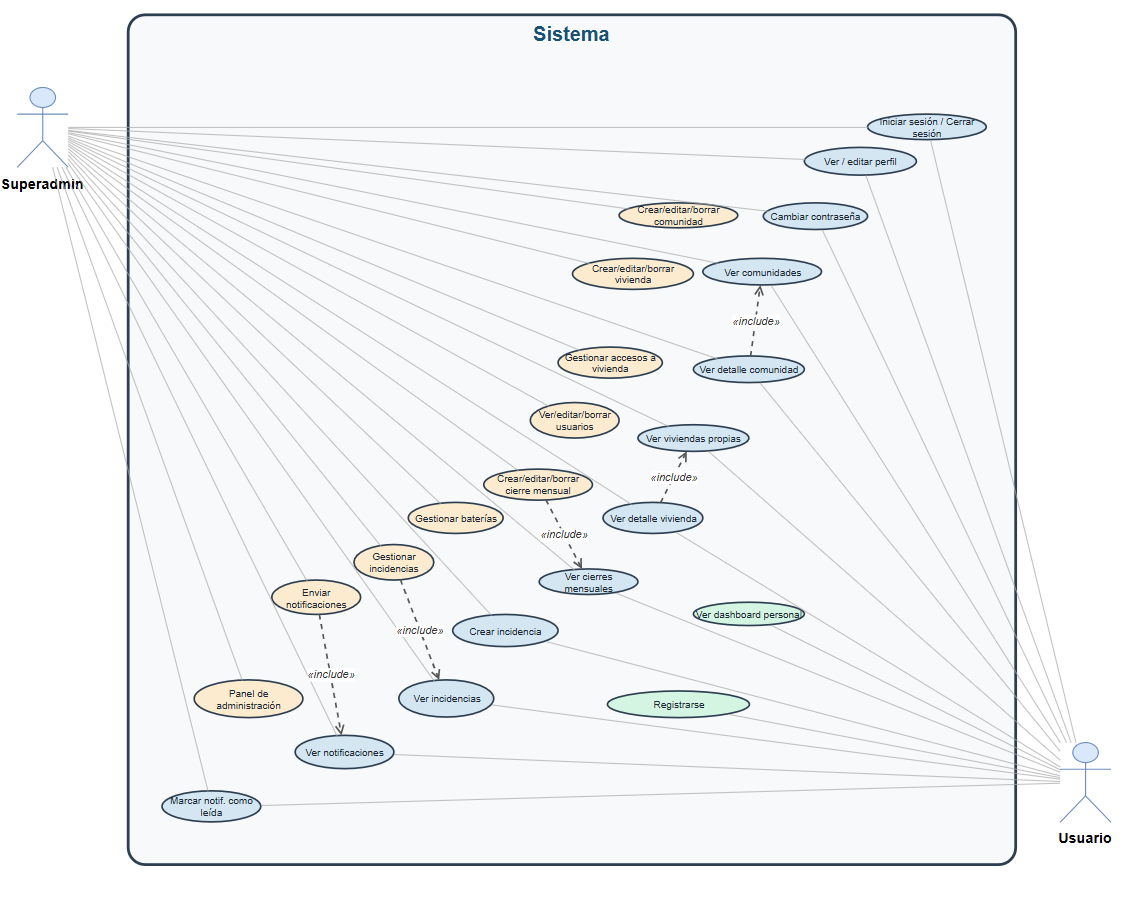
\includegraphics[width=0.95\textwidth]{img/casos_uso_saas.png}
  \caption{Diagrama de casos de uso de la plataforma SaaS (roles Superadmin
  y Usuario).}
  \label{fig:casos_uso}
\end{figure}

\subsection{Arquitectura}

La aplicación se organiza en \textit{blueprints} de Flask, uno por dominio
funcional. Los módulos principales gestionan las comunidades, las viviendas, los
cierres mensuales, las baterías, las notificaciones, las incidencias y los
accesos por rol. La persistencia recae en PostgreSQL, y el despliegue completo
(aplicación web, base de datos y proceso de inicialización de datos) se orquesta
con \texttt{docker-compose.yml}, un \texttt{Dockerfile} y un script
\texttt{entrypoint.sh}. Un endpoint \texttt{/health} permite a Docker Compose
verificar la disponibilidad del servicio mediante
\texttt{depends\_on: service\_healthy}.

\textbf{Modelo de datos.} El esquema se compone de siete entidades (ocho clases,
al modelarse \texttt{AccesoVivienda} como entidad asociativa), recogidas en la
Figura~\ref{fig:modelo_datos}. \texttt{Comunidad} agrupa sus \texttt{Vivienda}s
(1:N) y a lo sumo una \texttt{Bateria} (1:0..1); la relación entre
\texttt{Usuario} y \texttt{Vivienda} es N:M y se materializa en
\texttt{AccesoVivienda}, que almacena además el rol del usuario dentro de la
vivienda (titular, convivente o solo lectura). Cada \texttt{Vivienda} acumula su
histórico de \texttt{CierreMensual}, mientras que \texttt{Incidencia} y
\texttt{Notificacion} vinculan a los usuarios con sus comunidades y viviendas. El
acceso se diferencia en dos roles globales: \textbf{Superadmin}, que administra
el conjunto de entidades, y \textbf{Usuario}, con acceso restringido a sus
propias viviendas y cierres.

\begin{figure}[H]
  \centering
  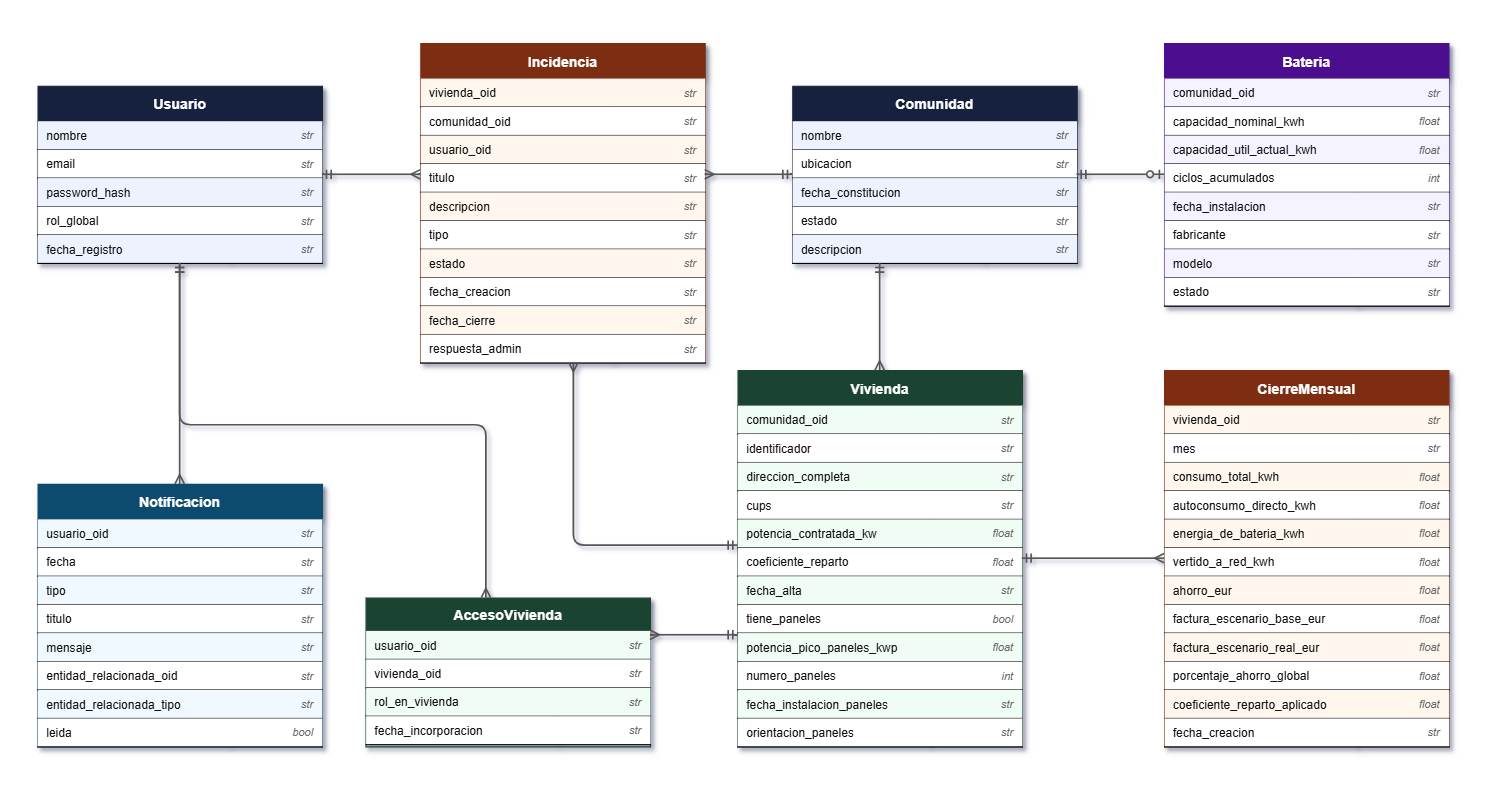
\includegraphics[width=\textwidth]{img/modelo_datos.png}
  \caption{Modelo de datos de la plataforma SaaS: siete entidades con
  \texttt{AccesoVivienda} como relación asociativa N:M entre \texttt{Usuario}
  y \texttt{Vivienda}.}
  \label{fig:modelo_datos}
\end{figure}

\subsection{Integración con el Motor de Decisión: la API Edge}

El nexo entre el modelo ONNX desplegado en el borde y la plataforma SaaS es la
API edge. El dispositivo de borde, tras ejecutar el controlador, comunica sus
decisiones y resultados a la plataforma a través de dos endpoints:
\texttt{/api/edge/decision}, que registra la decisión de carga/descarga de cada
hora, y \texttt{/api/edge/generar-cierre}, que dispara el cálculo del cierre
mensual. Ambos se autentican mediante un \textit{token} Bearer y están exentos
de la protección CSRF que aplica al resto de la aplicación, al ser consumidos
por un cliente automático y no por un navegador.

\subsection{Cálculo de Cierres y Reparto por Vivienda}
\label{sub:cierres}

El modelo de decisión opera sobre el agregado comunitario: el MPC y el Residual
SAC toman decisiones sobre la batería mirando el balance total de la comunidad
(consumo y generación totales), porque bajo el modelo de cooperativa con un único
punto de suministro (autoconsumo individual, Capítulo~\ref{chap:antecedentes}) el
balance agregado es la \textbf{única factura eléctrica oficial}. Por ello, el dato
primario del sistema es el agregado, y el desglose por vivienda no es una
facturación regulada, sino la \textbf{cuota interna} de reparto del gasto común
que la cooperativa asigna a cada socio. Este reparto se efectúa de forma
multiplicativa sobre el total horario: el consumo y la generación imputados a cada
vivienda se obtienen ponderando el total de la comunidad por el peso de la
vivienda (su potencia contratada para el consumo y su número de paneles para la
generación), de modo que la suma de las cuotas reproduce exactamente el total de
la factura común. Esta separación entre agregado (que ve el modelo) y desglose
(que ve el usuario) garantiza que la capa de presentación nunca altera los datos
sobre los que se entrenó y evaluó el controlador.

Esta elección de operar sobre el agregado no es solo una conveniencia de
modelado, sino una consecuencia de la observabilidad real del sistema. El
controlador, situado en el punto de generación y almacenamiento, solo mide en
tiempo real la generación fotovoltaica, el estado de carga de la batería y el
intercambio neto con la red en ese punto; el consumo de la comunidad no se mide
directamente en tiempo real —cada vivienda dispone, a lo sumo, de su propio
subcontador interno—, sino que se estima mediante previsión (perfil histórico agregado
y pronóstico meteorológico), que es precisamente la información que el motor
recibe en su ventana de pronóstico de 24~horas (Sección~\ref{sec:motor}). El
motor decide la acción de cada hora a partir de ese pronóstico —la hora en curso
es el primer paso de previsión, con la menor incertidumbre—, no del valor
realizado, que solo interviene en la liquidación física; de este modo se evita
cualquier anticipación de información (\textit{lookahead}) y tanto el MPC como el
agente reciben exactamente las mismas entradas, lo que garantiza una comparación
justa. El
desglose individualizado por vivienda solo se determina a posteriori, en el
reparto interno del gasto común entre los socios. Por ello, la política de la
batería se optimiza necesariamente sobre el balance agregado previsto, y el
reparto por participante es competencia de la liquidación interna posterior y no
del control.

El \textbf{escenario de referencia} para medir el ahorro corresponde al coste
que tendría cada vivienda con sus propios paneles fotovoltaicos pero sin batería
comunitaria ni reparto colectivo. Para cada hora $h$:
\begin{align}
  \text{compra\_base}_h &= \max(0,\; c_h - g_h) \cdot p_c^h \\
  \text{comp\_base}_h   &= \max(0,\; g_h - c_h) \cdot p_v^h
\end{align}
donde $c_h$ y $g_h$ son el consumo y la generación individuales de la vivienda.
La factura de referencia mensual es
$\text{factura\_base} = \max(0, \sum_h \text{compra\_base}_h -
\sum_h \text{comp\_base}_h)$, y el ahorro mide el valor añadido de la comunidad
(batería más reparto colectivo) sobre el autoconsumo individual con paneles
propios: $\text{ahorro} = \max(0, \text{factura\_base} - \text{factura\_real})$.
Comparar contra el escenario \textit{con paneles propios} (y no contra el
escenario sin ningún sistema solar) aísla el valor que aporta específicamente la
batería comunitaria y el reparto, evitando atribuirle el ahorro que ya
proporcionarían los paneles individuales por sí solos.

\subsection{Naturaleza de los Valores del Panel de Control}
\label{sub:panel}

Los valores económicos mostrados en el panel de control de la plataforma (ahorro
mensual y acumulado por vivienda) provienen de una simulación de operación
continua sobre datos históricos consecutivos, cuyo propósito es demostrar la
integración completa del sistema de extremo a extremo. \textbf{No constituyen
una evaluación del modelo}, que se realiza exclusivamente sobre el conjunto de
evaluación \textit{held-out} de 50 semanas según se detalla en la
Sección~\ref{sub:resultados}. Esta distinción es importante: el panel ilustra el
funcionamiento del sistema desplegado, mientras que la validación científica del
controlador reside en el protocolo de evaluación reproducible.

% ==============================================================
\chapter{Planificación y Seguimiento}
\label{chap:planificacion}
% ==============================================================

\section{Fases del Proyecto}

\begin{table}[H]
\centering
\caption{Fases del proyecto y distribución temporal.}
\label{tab:fases}
\begin{tabularx}{\textwidth}{C{0.5cm}L{4.2cm}C{1.8cm}C{1.8cm}}
\toprule
\textbf{\#} & \textbf{Fase} & \textbf{Inicio} & \textbf{Fin} \\
\midrule
0 & Concepción y viabilidad & Sep 2024 & Oct 2024 \\
1 & Setup, arquitectura, YAML & Oct 2024 & Nov 2024 \\
2 & Ingeniería de datos (ETL) & Nov 2024 & Dic 2024 \\
3 & Simulador físico-económico & Dic 2024 & Ene 2025 \\
4 & Controlador MPC & Ene 2025 & Feb 2025 \\
5 & Experimentación DQN y PPO & Feb 2025 & Mar 2025 \\
6 & Residual SAC y tuning & Mar 2025 & May 2025 \\
7 & Evaluación unificada y API & May 2025 & Jun 2025 \\
8 & Documentación y defensa & Jun 2025 & Jul 2025 \\
\bottomrule
\end{tabularx}
\end{table}

\begin{figure}[H]
  \centering
  \figpend[0.95\textwidth]{[Figura: Diagrama de Gantt planificado vs.\ real]\\
    \textit{Fases 0--8. Barra gris: planificado. Barra color: real.}}
  \caption{Diagrama de Gantt del proyecto.}
  \label{fig:gantt}
\end{figure}

\section{Desviaciones Técnicas}

Las fases 5 y 6 acumularon la mayor desviación. La Fase~5 se alargó porque
los experimentos con DQN y PPO requirieron análisis sistemático adicional
para entender las causas del bajo rendimiento antes del descarte documentado.
La Fase~6 se alargó por tres causas: (1) la \textit{cold-start pathology},
identificada y resuelta mediante el protocolo de pre-llenado; (2) el diseño
iterativo del espacio de observación de 112 dimensiones; y (3) el tuning de
$\delta_{\max}$ y \texttt{ent\_coef} mediante exploración sistemática con
TensorBoard.

% ==============================================================
\chapter{Principales Aportaciones}
\label{chap:aportaciones}
% ==============================================================

\textbf{Aportación 1 — Proceso documentado de selección del algoritmo de RL
(OG-1, OG-3).} A diferencia de trabajos que implementan directamente el
algoritmo de moda, este trabajo documenta la experimentación con DQN y PPO,
el análisis de sus limitaciones estructurales y el diseño del Residual SAC
que las resuelve. La comparativa con un MPC realista bien calibrado como
\textit{baseline} (en lugar de una heurística simple) sitúa los resultados
en el contexto del estado del arte.

\textbf{Aportación 2 — Gemelo digital calibrado con datos reales (OG-2).}
Un simulador físico-económico con modelo de degradación no lineal LFP,
modelo económico asimétrico coherente con el RD 244/2019 y dataset de
22.646 horas construido a partir de fuentes oficiales. La brecha intencional
entre la degradación linealizada del MPC y el modelo no lineal del simulador
es la base del margen de mejora que el Residual SAC explota.

\textbf{Aportación 3 — Instanciación de la arquitectura Residual RL en el
almacenamiento comunitario, con garantía de suelo exacta y verificada (OG-3).}
El paradigma del aprendizaje residual sobre un controlador base no es original
de este trabajo: lo propusieron \citet{Johannink2019} en el contexto del control
robótico. La aportación concreta es su adaptación al dominio de la batería
comunitaria: un agente SAC que corrige a un MPC realista mediante una
formulación residual \textbf{multiplicativa},
$\text{flow}\times(1+\Delta\cdot\delta_{\max})$ con $\delta_{\max}=0{,}15$, a la
que se llegó tras descartar empíricamente la variante aditiva del trabajo
original (Sección~\ref{sub:residual_sac}). Frente a la formulación aditiva, esta
escala la corrección con la magnitud del flujo del MPC y, sobre todo, hace que
la propiedad de suelo sea \textbf{exacta}: con $\Delta = \mathbf{0}$,
$\text{flow}\times(1+0)=\text{flow}$, de modo que el peor caso del motor es
exactamente el MPC realista. Esta propiedad se verifica empíricamente con el
test \texttt{test\_delta\_zero\_matches\_mpc} (módulo
\texttt{test\_residual\_env.py}) y no la ofrece ningún algoritmo de RL puro.

\textbf{Aportación 4 — Plataforma abierta para comunidades rurales (OG-4).}
Una plataforma software basada íntegramente en herramientas y fuentes de datos
públicas (ESIOS, PVGIS, Open-Meteo), con dashboards diferenciados por rol que
democratizan el acceso a la gestión energética inteligente para comunidades de
pequeña escala sin conocimientos técnicos.

% ==============================================================
\chapter{Conclusiones}
\label{chap:conclusiones}
% ==============================================================

\section{Conclusiones Técnicas}

El trabajo demuestra empíricamente que RL puro no supera al MPC realista de
forma consistente en el dominio de la gestión de baterías comunitarias, resultado
coherente con la literatura reciente \citep{Zhan2023}. DQN sufre un error de
cuantización estructural irresolvible con el espacio discreto de 9 acciones,
y PPO no puede aprovechar el protocolo de inicialización con demostraciones por
su naturaleza \textit{on-policy}.

La arquitectura Residual SAC resuelve ambas limitaciones: opera en espacio
continuo y se inicializa con demostraciones del MPC, eliminando la
\textit{cold-start pathology}. La propiedad de garantía de suelo —que el
sistema no puede rendir peor que el MPC realista— es la contribución técnica
más valiosa de la arquitectura residual.

El MPC realista alcanza $+47{,}64$\,€/semana respecto a IDLE,
con un margen teórico de mejora de $9{,}00$\,€/semana (15{,}9\,\%) disponible
para el Residual SAC. La cuantificación explícita de este margen permite
contextualizar los resultados sin sobreestimar el potencial del RL en este
dominio.

\section{Limitaciones y Decisiones de Diseño}
\label{sec:limitaciones}

El alcance de este trabajo conlleva simplificaciones que conviene explicitar,
distinguiendo las decisiones de diseño deliberadas de las limitaciones impuestas
por los datos disponibles.

\textbf{Optimización sobre el balance agregado y modelo de comunidad.} El
controlador optimiza el beneficio económico sobre el \textbf{balance agregado} de
la comunidad. Bajo el modelo adoptado —cooperativa con un único punto de
suministro, en la modalidad de autoconsumo individual
(Capítulo~\ref{chap:antecedentes})— ese balance agregado \emph{es} la única
factura eléctrica oficial, por lo que la optimización del agregado se corresponde
\textbf{exactamente} con el coste real, sin desfase entre el objetivo del control
y la liquidación. La decisión es además coherente con la observabilidad del
sistema: la batería es un único activo físico compartido cuya política de carga y
descarga depende solo del balance neto comunitario, y el controlador local
únicamente observa magnitudes agregadas previstas (Sección~\ref{sub:cierres}),
pues el consumo individualizado solo está disponible a posteriori.

La \textbf{condición de aplicabilidad} de este modelo es disponer de un único
punto de suministro (contador frontera) sobre una \textbf{red interior privada}.
Esto es realista en la ecocomunidad rural adoptada —parcelas colindantes de
titularidad privada, sin vía de dominio público interpuesta, con la cooperativa
como titular único del suministro y subcontadores internos para el reparto del
gasto común (Sección~\ref{sec:marco_regulatorio})—, pero no en un conjunto de
viviendas independientes con CUPS propios y separadas por viario público, donde
no es legal tender cableado privado y cada vecino conserva su comercializadora.
Conviene además ser explícito en que esta configuración \emph{no} es una figura
regulada estándar (las Redes de Distribución Cerradas del RD 1183/2020 y RD
314/2023 se reservan a entornos industriales): se sostiene como red interior de un
único consumidor, lo que exige la renuncia de los vecinos al contrato individual.
En el escenario alternativo —viviendas independientes— la comunidad operaría en
\textbf{autoconsumo colectivo}, con factura individual por coeficientes; entonces
el balance agregado deja de ser la factura y queda como capa de control, y la suma
de las facturas individuales podría diferir del óptimo agregado al no existir
compensación cruzada entre vecinos en la misma hora.
Reconciliar ambas capas con una recompensa formulada vivienda a vivienda afinaría
el momento de descarga según el encaje horario de cada perfil, pero exigiría
datos de consumo individualizados en tiempo real de los que ni el prototipo ni un
despliegue estándar disponen, por lo que entrenarla sobre los perfiles sintéticos
actuales conduciría a sobreajuste.

\textbf{Naturaleza sintética de los datos.} El dataset es un agregado
representativo construido a partir del perfil normalizado 2.0TD de ESIOS escalado
al consumo medio del hogar español, no un registro de quince viviendas reales; el
desglose por vivienda de la capa de facturación es, en consecuencia, una
proyección sintética. Los resultados son válidos bajo las hipótesis del modelo y
no constituyen mediciones de una instalación física.

\textbf{Especialización a la comunidad de estudio.} El controlador residual aprende
sobre el perfil concreto de la comunidad modelada (quince viviendas, \SI{42}{kWp},
batería de \SI{80}{kWh}); trasladarlo a otra comunidad de distinto tamaño,
generación o consumo exige regenerar el dataset y reentrenar, pues la política se
ajusta a esa distribución de carga y generación. No obstante, el \textbf{MPC base
opera sin reentrenamiento} sobre cualquier comunidad, pues resuelve su \acrshort{lp}
con los datos que reciba, de modo que el sistema \textbf{degrada de forma controlada}:
ante una comunidad no vista, el peor caso es operar con el MPC realista mientras se
reentrena el residual. Un ajuste fino por comunidad (\textit{transfer learning})
queda como línea de trabajo futuro (Capítulo~\ref{chap:futuro}).

\textbf{Modelo de degradación.} La degradación se modela como un coste en la
función de recompensa que induce un uso conservador del almacenamiento, pero no
reduce la capacidad útil a lo largo del episodio; el efecto del envejecimiento
sobre la vida útil se traslada al análisis de viabilidad económica mediante el
coste de capital amortizado (Anexo~\ref{app:viabilidad}). Asimismo, solo se
contabiliza el envejecimiento por \emph{ciclado} (proporcional a la energía
movida, dominante en una batería de uso diario); el envejecimiento de
\emph{calendario} —degradación por tiempo y temperatura, independiente del uso—
queda fuera del alcance del modelo. Además, el coste de
degradación efectivo ($\approx0{,}006$\,€/kWh, Sección~\ref{sub:calibracion-degradacion})
se calibra a la amortización de una batería LFP \emph{subvencionada}; bajo un
coste no subvencionado el ahorro absoluto reportado sería algo menor. En todo
caso, al aplicarse de forma idéntica a todos los controladores, la comparación
entre ellos —objeto del estudio— es invariante a su valor.

\textbf{Marco regulatorio en evolución.} El tratamiento normativo del
almacenamiento compartido se encuentra en evolución: junto al Real Decreto-ley
7/2025, en 2025 se ha sometido a consulta pública un proyecto de real decreto
específico sobre el almacenamiento en autoconsumo colectivo. Por su carácter de
norma en tramitación, no se asume aquí como marco vigente; su eventual aprobación
podría refinar el tratamiento del reparto de la energía
almacenada.\footnote{Referencia normativa pendiente de confirmación una vez
publicada la norma definitiva en el BOE.}

\section{Conclusiones Personales}

La principal lección del trabajo es que el rigor en la construcción del entorno
de simulación es tan importante como la sofisticación del algoritmo de RL. Un
simulador con invariantes violados —simultaneidad de carga y descarga, data
leakage en el split, SoC fuera de rango— invalida cualquier resultado
independientemente de la complejidad del agente. La suite de 47 tests
automatizados no es documentación, es parte del resultado.

La segunda lección es el valor de documentar los experimentos fallidos. El
análisis de por qué DQN y PPO no funcionan en este dominio —identificando el
error de cuantización y la incompatibilidad \textit{on-policy}— tiene mayor
valor académico que simplemente presentar el resultado del algoritmo ganador.
Un experimento con resultado negativo bien analizado justifica las decisiones
de diseño del algoritmo final.

% ==============================================================
\chapter{Líneas de Trabajo Futuro}
\label{chap:futuro}
% ==============================================================

El \textbf{aumento del número de semillas de evaluación} (de 3 a 10) es el
refinamiento inmediato sobre los resultados ya obtenidos con la configuración
final: estrecharía el intervalo de confianza de la mejora del Residual SAC sobre
el MPC y permitiría un contraste de significancia formal (por ejemplo, un test
de Wilcoxon emparejado por semana).

La \textbf{activación de APIs en tiempo real} es la extensión natural: los
conectores ESIOS, Open-Meteo y datadis se diseñan con la misma interfaz que el
dataset histórico; activarlos requiere configurar los tokens de acceso.

El \textbf{despliegue en hardware de borde} (Raspberry Pi con interfaz Modbus
al inversor) es el paso hacia la operación real de los Niveles~1 y~2 del
control jerárquico. La arquitectura MPC+Residual SAC tiene una ventaja clave:
el MPC base opera desde el primer día sin reentrenamiento.

La \textbf{participación en mercados intradiarios de OMIE} y servicios de
balance de REE ampliaría la plataforma hacia una arquitectura de gestión
energética multi-capa, cubriendo los horizontes sub-horarios de 15 minutos a
2 horas.

Los \textbf{coeficientes de reparto dinámicos} ($\beta_{i,h}$ variables hora
a hora) son la extensión de mayor impacto económico, requiriendo modelado
individual por vivienda y un módulo de liquidación más complejo.

La \textbf{previsión con modelos LSTM} para irradiancia y consumo podría
reducir el coste del ruido de pronóstico ($9{,}00$\,€/semana) y ampliar el
margen disponible para el Residual SAC.

% ── REFERENCIAS ───────────────────────────────────────────────
\bibliography{referencias}

% ── ANEXOS ────────────────────────────────────────────────────
\appendix

\chapter{Capacidad Fotovoltaica por Vivienda}
\label{app:capacidad}

La Tabla~\ref{tab:capacidad} recoge la capacidad fotovoltaica instalada en cada
una de las quince viviendas de la comunidad Vilarín, registrada en la plataforma
SaaS y utilizada como base para el reparto de la generación. Cada panel tiene
una potencia de \SI{400}{Wp} (silicio monocristalino, orientación sur,
inclinación óptima). Las capacidades individuales suman exactamente \SI{42}{kWp}.

\begin{table}[H]
\centering
\caption{Capacidad fotovoltaica y número de paneles por vivienda.}
\label{tab:capacidad}
\begin{tabular}{llrr}
\toprule
\textbf{Código} & \textbf{Dirección} & \textbf{kWp} & \textbf{Paneles} \\
\midrule
I001 & Rúa da Igrexa 1 & 2{,}4 & 6 \\
I002 & Rúa da Igrexa 3 & 2{,}4 & 6 \\
I003 & Rúa da Igrexa 5 & 2{,}0 & 5 \\
I004 & Rúa da Igrexa 7 & 2{,}0 & 5 \\
I005 & Rúa da Igrexa 9 & 3{,}2 & 8 \\
I006 & Rúa da Igrexa 11 & 2{,}0 & 5 \\
R001 & Camiño do Río 2 & 4{,}4 & 11 \\
R002 & Camiño do Río 4 & 2{,}8 & 7 \\
R003 & Camiño do Río 6 & 2{,}0 & 5 \\
R004 & Camiño do Río 8 & 2{,}4 & 6 \\
R005 & Camiño do Río 10 & 5{,}2 & 13 \\
R006 & Camiño do Río 12 & 2{,}8 & 7 \\
O001 & Lugar de Outeiro 1 & 2{,}4 & 6 \\
O002 & Lugar de Outeiro 3 & 2{,}4 & 6 \\
O003 & Lugar de Outeiro 5 & 3{,}6 & 9 \\
\midrule
\textbf{Total} & & \textbf{42{,}0} & \textbf{105} \\
\bottomrule
\end{tabular}
\end{table}

\chapter{Configuración Completa: system.yaml}
\label{app:config}
[Espacio reservado para el fichero \texttt{config/system.yaml} completo con
todos los hiperparámetros del sistema.]

\chapter{Árbol de Directorios del Repositorio}
\label{app:estructura}
[Espacio reservado para el árbol completo de directorios con descripción de
cada módulo.]

\chapter{Suite de Tests Automatizados}
\label{app:tests}

Los 47 tests automatizados ejecutables con \texttt{pytest} se distribuyen en
cinco módulos: \texttt{test\_dataset.py} (12 tests del pipeline ETL),
\texttt{test\_energy\_env\_continuo.py} (16 tests del entorno y el simulador),
\texttt{test\_mpc.py} (7 tests del controlador MPC),
\texttt{test\_residual\_env.py} (10 tests de la arquitectura residual) y
\texttt{test\_delta\_zero.py} (2 tests de la propiedad de suelo). El
Cuadro~\ref{tab:tests} recoge una selección de los invariantes críticos
verificados:

\begin{table}[H]
\centering
\caption{Tests críticos del sistema.}
\label{tab:tests}
\begin{tabularx}{\textwidth}{lXl}
\toprule
\textbf{Test} & \textbf{Propósito} & \textbf{Módulo} \\
\midrule
\texttt{test\_split\_no\_solapado} & Pools train/eval completamente disjuntos & ETL \\
\texttt{test\_delta\_zero\_matches\_mpc} & $\Delta=\mathbf{0}$ $\Rightarrow$ replica al MPC realista & Residual \\
\texttt{test\_residual\_delta\_zero} & Salida nula del actor preserva la acción MPC & Residual \\
\texttt{test\_soc\_always\_in\_bounds} & SoC $\in [10\%, 90\%]$ en todo momento & Simulador \\
\texttt{test\_soc\_max\_no\_carga} & No carga por encima del SoC máximo & Simulador \\
\texttt{test\_soc\_min\_no\_descarga} & No descarga por debajo del SoC mínimo & Simulador \\
\texttt{test\_precios\_excedente\_no\_negativos} & $p_{\text{exc}} \geq 0$ en todo el dataset & ETL \\
\bottomrule
\end{tabularx}
\end{table}

\chapter{Análisis de Viabilidad Económica}
\label{app:viabilidad}

\section{Coste de la Inversión}

El coste de un sistema de almacenamiento BESS comercial LFP de \SI{80}{kWh} en
formato armario se sitúa, según las referencias de mercado de 2026, en un rango
de 180 a 300 €/kWh para sistemas instalados de esta escala. Tomando un valor de
referencia de 250\,€/kWh para una instalación de pequeña escala (más cara
por kWh que los grandes proyectos de red), la inversión asciende a
aproximadamente 20.000\,€.

\section{Beneficio del Controlador y Periodo de Retorno}

El beneficio económico que sustenta este análisis es el beneficio marginal
validado del controlador frente al escenario sin batería (IDLE):
$+48{,}35$\,€/semana sobre el conjunto de evaluación
(Sección~\ref{sub:resultados}), equivalente a unos 2.500\,€/año para el
conjunto de la comunidad. Representa el valor marginal real de la batería —el
desplazamiento temporal de energía que el controlador optimiza—, independiente
del autoconsumo solar directo, que es atribuible a los paneles y no al
almacenamiento. Conviene matizar que esta cifra refleja el régimen de precios del
periodo 2021--2023, que incluye la crisis energética de 2022; en un escenario de
precios más moderados el beneficio anual sería menor.

Conviene subrayar esta distinción, recurrente en el análisis del sistema: el
grueso del ahorro de una instalación de autoconsumo procede de consumir la
energía solar en el momento de generarla, lo que ocurre con o sin batería. La
batería únicamente añade el desplazamiento temporal de los excedentes, y es ese
desplazamiento lo que el controlador optimiza y la simulación cuantifica.

\begin{center}
\fbox{\parbox{0.95\textwidth}{\small \textbf{Nota.} Este análisis parte del
beneficio marginal validado del controlador ($+48{,}35$\,€/semana,
Sección~\ref{sub:resultados}) y constituye una estimación de orden de magnitud.
No debe confundirse con los valores por vivienda en €/año que ilustra el panel de
la plataforma (Sección~\ref{sub:panel}), procedentes de una simulación de
facturación de extremo a extremo con un propósito distinto.}}
\end{center}

Con una inversión de referencia de 20.000\,€ (250\,€/kWh
$\times$ \SI{80}{kWh}) y un beneficio anual del orden de 2.500\,€, el periodo
de retorno simple sin ayudas se sitúa en torno a los ocho años, frente a una vida
útil de la batería LFP de 15 a 20 años. Es, por tanto, una inversión de retorno
positivo aunque ajustado en ausencia de ayudas públicas.

\section{El Papel de las Subvenciones}

El marco de ayudas vigente en España modifica sustancialmente esta conclusión.
La segunda convocatoria del Programa de Energías Renovables Innovadoras del IDAE
incluye un programa específico de autoconsumo colectivo con almacenamiento,
dotado con 368,5 millones de euros, en el que las comunidades de propietarios
son elegibles, con una intensidad de ayuda del 40\,\% a fondo perdido. A esto se
suma la deducción en el IRPF por reformas de mejora de la eficiencia energética
(RD-ley 19/2021, prorrogado) y bonificaciones municipales en el IBI.

Aplicando una subvención del 40\,\%, la inversión neta desciende a unos
12.000\,€, lo que reduce el periodo de retorno a aproximadamente cinco años,
holgadamente dentro de la vida útil del sistema.

\section{Conclusión}

El análisis arroja una conclusión honesta y matizada: el beneficio del
almacenamiento gestionado hace de la batería una inversión de retorno positivo
aunque ajustado sin ayudas públicas (en torno a ocho años), que el marco de
subvención actualmente vigente y dotado convierte en claramente rentable. Esta
dependencia de las ayudas no es una particularidad del proyecto, sino la
realidad de prácticamente todas las comunidades energéticas en España. En este
contexto, el valor del controlador inteligente es precisamente maximizar el
retorno disponible sea cual sea el escenario de ayudas, extrayendo el mayor
beneficio posible de la batería instalada. El dimensionamiento óptimo conjunto
de generación y almacenamiento, así como una política generalizable a distintas
capacidades, constituyen líneas de trabajo futuro.

\chapter{Historial Completo de Experimentos}
\label{app:historial}

Este anexo recoge el historial completo de configuraciones de agentes
entrenadas durante el desarrollo del motor de decisión. El cuerpo de la memoria
(Sección~\ref{sec:motor}) presenta únicamente los hitos representativos que
motivaron decisiones de diseño; este anexo documenta el volumen real de
experimentación, incluyendo configuraciones intermedias y fallidas, como
evidencia del proceso iterativo de tuning y justificación de las desviaciones
de planificación recogidas en el Capítulo~\ref{chap:planificacion}.

\section{Familia DQN}

\begin{table}[H]
\centering
\caption{Historial de configuraciones DQN.}
\label{tab:hist_dqn}
\small
\begin{tabularx}{\textwidth}{lL{1.4cm}L{1cm}L{1.3cm}L{1.2cm}L{1.3cm}X}
\toprule
\textbf{Ver.} & \textbf{Obs.} & \textbf{Acc.} & \textbf{n-step} &
\textbf{Buffer} & \textbf{Pasos} & \textbf{Resultado / Nota} \\
\midrule
DQN\_10 & 101 & 13 & 1 & 100k & 1M & Base, sin n-step ni AR(1) \\
DQN\_11 & 101 & 13 & 1 & 100k & 2M & $\approx$39{,}38; AR(1) añadido \\
DQN\_12 & 101 & 13$\to$9 & 8 & 200k & 2M & Interrumpido; reduce acciones \\
DQN\_13 & 101 & 9 & 8 & 200k & 1{,}88M & \textbf{+45{,}23} (mejor); $\gamma$=0{,}995 \\
DQN\_14 & 101 & 9 & 24 & 400k & 3M & +41{,}71; no convergió \\
DQN\_15 & 107 & 9 & 8 & 400k & 3M & Máx +51{,}83; buffer erróneo \\
DQN\_16 & 107 & 9 & 24 & 200k & 5M & Crash a 4M; datos perdidos \\
DQN\_17 & 101 & 9 & 24 & 200k & 5M & Run corto, abortado \\
DQN\_18 & 101 & 9 & 24 & 200k & 5M & 30--35; no converge \\
DQN\_19 & 107 & 9 & 8 & 200k & 3M & 30--35; no converge \\
DQN\_20 & 101 & 9 & 8 & 200k & 3M & \textbf{+45{,}07}; $\gamma$=0{,}99 \\
\bottomrule
\end{tabularx}
\end{table}

La conclusión de la familia DQN es que las configuraciones con $n=8$ (DQN\_13 y
DQN\_20) son las que mejor rinden, alcanzando ambas en torno a
$+45$\,€/semana pese a usar factores de descuento distintos ($\gamma=0{,}995$ y
$\gamma=0{,}99$ respectivamente). Las configuraciones DQN\_18 y DQN\_19 no
replicaron este rendimiento y se estancaron en torno a $30$--$35$\,€/semana, lo
que sugiere que la convergencia depende de la interacción entre el factor de
descuento, el número de pasos de propagación \textit{n-step} y la duración del
entrenamiento, y no de un único hiperparámetro de forma aislada. El conjunto de
experimentos confirma que la combinación $n=8$ con entrenamiento suficiente es
la vía más fiable hacia el mejor rendimiento de la familia.

\section{Familia PPO}

\begin{table}[H]
\centering
\caption{Historial de configuraciones PPO.}
\label{tab:hist_ppo}
\small
\begin{tabularx}{\textwidth}{lL{1.2cm}L{1.6cm}L{2.2cm}L{1cm}X}
\toprule
\textbf{Ver.} & \textbf{Obs.} & \textbf{Rollout} & \textbf{ent\_coef} &
\textbf{Pasos} & \textbf{Resultado / Nota} \\
\midrule
PPO\_1 & 101 & 2048 & 0{,}01 const. & 3M & Máx +39{,}91; colapso a 36 \\
PPO\_2 & 101 & 4096 & 0{,}003 const. & 3M & Máx +41{,}82; colapso a 37 \\
PPO\_3 & 108 & 8192 & decay 0{,}005$\to$0{,}0005 & 3M & +44{,}72; sin colapso \\
PPO\_4 & 108 & 8192 & decay + LR decay & 4M & \textbf{+45{,}69}; convergió \\
\bottomrule
\end{tabularx}
\end{table}

El decaimiento del coeficiente de entropía (PPO\_3, PPO\_4) resuelve el colapso
de política observado en las configuraciones con entropía constante (PPO\_1,
PPO\_2). PPO\_4 añade además decaimiento de la tasa de aprendizaje, logrando la
mejor configuración de la familia.

\section{Familia Residual SAC}

\begin{table}[H]
\centering
\caption{Historial de configuraciones Residual SAC.}
\label{tab:hist_sac}
\small
\begin{tabularx}{\textwidth}{lL{2cm}L{1.3cm}L{1.2cm}L{1.3cm}X}
\toprule
\textbf{Ver.} & \textbf{Arquit.} & \textbf{$\delta_{\max}$} &
\textbf{ent} & \textbf{Warmup} & \textbf{Resultado / Nota} \\
\midrule
v2 & aditiva & 0{,}10 & 0{,}01 & 50k & +48{,}80; sin neteo, OOM \\
v3 & aditiva & 0{,}05 & 0{,}005 & 50k & $\approx$41; correcciones mínimas \\
v4 & multiplic. & 0{,}30 & 0{,}002 & 100k & $\approx$43{,}3; se estanca \\
\textbf{v5} & \textbf{multiplic.} & \textbf{0{,}15} & \textbf{0{,}01} &
\textbf{100k} & \textbf{+49{,}23; supera MPC} \\
v5b & multiplic. & 0{,}20 & 0{,}01 & 100k & +49{,}06; rango amplio peor \\
v5c & multiplic. & 0{,}15 & 0{,}01 & 200k & Warmup doble; en curso \\
\bottomrule
\end{tabularx}
\end{table}

La progresión de la familia Residual SAC ilustra el proceso de refinamiento de
la arquitectura: la transición de aditiva (v2, v3) a multiplicativa (v4--v5c)
resuelve el problema de la corrección de magnitud fija, y el ajuste del rango
de corrección de $\delta_{\max} = 0{,}30$ (v4) a $0{,}15$ (v5) consigue el
equilibrio entre capacidad de corrección y respeto a la política base del MPC.
La configuración v5 es la seleccionada y, una vez fijado el dimensionado
definitivo, se reentrenó sobre \SI{42}{kWp}/\SI{80}{kWh} (versión v6), cuyos
resultados son los reportados en la Sección~\ref{sub:resultados}.

\end{document}
